
\documentclass{article} % For LaTeX2e
\usepackage{iclr2023_conference,times}

% Optional math commands from https://github.com/goodfeli/dlbook_notation.
%%%%% NEW MATH DEFINITIONS %%%%%

\usepackage{amsmath,amsfonts,bm}

% Mark sections of captions for referring to divisions of figures
\newcommand{\figleft}{{\em (Left)}}
\newcommand{\figcenter}{{\em (Center)}}
\newcommand{\figright}{{\em (Right)}}
\newcommand{\figtop}{{\em (Top)}}
\newcommand{\figbottom}{{\em (Bottom)}}
\newcommand{\captiona}{{\em (a)}}
\newcommand{\captionb}{{\em (b)}}
\newcommand{\captionc}{{\em (c)}}
\newcommand{\captiond}{{\em (d)}}

% Highlight a newly defined term
\newcommand{\newterm}[1]{{\bf #1}}


% Figure reference, lower-case.
\def\figref#1{figure~\ref{#1}}
% Figure reference, capital. For start of sentence
\def\Figref#1{Figure~\ref{#1}}
\def\twofigref#1#2{figures \ref{#1} and \ref{#2}}
\def\quadfigref#1#2#3#4{figures \ref{#1}, \ref{#2}, \ref{#3} and \ref{#4}}
% Section reference, lower-case.
\def\secref#1{section~\ref{#1}}
% Section reference, capital.
\def\Secref#1{Section~\ref{#1}}
% Reference to two sections.
\def\twosecrefs#1#2{sections \ref{#1} and \ref{#2}}
% Reference to three sections.
\def\secrefs#1#2#3{sections \ref{#1}, \ref{#2} and \ref{#3}}
% Reference to an equation, lower-case.
\def\eqref#1{equation~\ref{#1}}
% Reference to an equation, upper case
\def\Eqref#1{Equation~\ref{#1}}
% A raw reference to an equation---avoid using if possible
\def\plaineqref#1{\ref{#1}}
% Reference to a chapter, lower-case.
\def\chapref#1{chapter~\ref{#1}}
% Reference to an equation, upper case.
\def\Chapref#1{Chapter~\ref{#1}}
% Reference to a range of chapters
\def\rangechapref#1#2{chapters\ref{#1}--\ref{#2}}
% Reference to an algorithm, lower-case.
\def\algref#1{algorithm~\ref{#1}}
% Reference to an algorithm, upper case.
\def\Algref#1{Algorithm~\ref{#1}}
\def\twoalgref#1#2{algorithms \ref{#1} and \ref{#2}}
\def\Twoalgref#1#2{Algorithms \ref{#1} and \ref{#2}}
% Reference to a part, lower case
\def\partref#1{part~\ref{#1}}
% Reference to a part, upper case
\def\Partref#1{Part~\ref{#1}}
\def\twopartref#1#2{parts \ref{#1} and \ref{#2}}

\def\ceil#1{\lceil #1 \rceil}
\def\floor#1{\lfloor #1 \rfloor}
\def\1{\bm{1}}
\newcommand{\train}{\mathcal{D}}
\newcommand{\valid}{\mathcal{D_{\mathrm{valid}}}}
\newcommand{\test}{\mathcal{D_{\mathrm{test}}}}

\def\eps{{\epsilon}}


% Random variables
\def\reta{{\textnormal{$\eta$}}}
\def\ra{{\textnormal{a}}}
\def\rb{{\textnormal{b}}}
\def\rc{{\textnormal{c}}}
\def\rd{{\textnormal{d}}}
\def\re{{\textnormal{e}}}
\def\rf{{\textnormal{f}}}
\def\rg{{\textnormal{g}}}
\def\rh{{\textnormal{h}}}
\def\ri{{\textnormal{i}}}
\def\rj{{\textnormal{j}}}
\def\rk{{\textnormal{k}}}
\def\rl{{\textnormal{l}}}
% rm is already a command, just don't name any random variables m
\def\rn{{\textnormal{n}}}
\def\ro{{\textnormal{o}}}
\def\rp{{\textnormal{p}}}
\def\rq{{\textnormal{q}}}
\def\rr{{\textnormal{r}}}
\def\rs{{\textnormal{s}}}
\def\rt{{\textnormal{t}}}
\def\ru{{\textnormal{u}}}
\def\rv{{\textnormal{v}}}
\def\rw{{\textnormal{w}}}
\def\rx{{\textnormal{x}}}
\def\ry{{\textnormal{y}}}
\def\rz{{\textnormal{z}}}

% Random vectors
\def\rvepsilon{{\mathbf{\epsilon}}}
\def\rvtheta{{\mathbf{\theta}}}
\def\rva{{\mathbf{a}}}
\def\rvb{{\mathbf{b}}}
\def\rvc{{\mathbf{c}}}
\def\rvd{{\mathbf{d}}}
\def\rve{{\mathbf{e}}}
\def\rvf{{\mathbf{f}}}
\def\rvg{{\mathbf{g}}}
\def\rvh{{\mathbf{h}}}
\def\rvu{{\mathbf{i}}}
\def\rvj{{\mathbf{j}}}
\def\rvk{{\mathbf{k}}}
\def\rvl{{\mathbf{l}}}
\def\rvm{{\mathbf{m}}}
\def\rvn{{\mathbf{n}}}
\def\rvo{{\mathbf{o}}}
\def\rvp{{\mathbf{p}}}
\def\rvq{{\mathbf{q}}}
\def\rvr{{\mathbf{r}}}
\def\rvs{{\mathbf{s}}}
\def\rvt{{\mathbf{t}}}
\def\rvu{{\mathbf{u}}}
\def\rvv{{\mathbf{v}}}
\def\rvw{{\mathbf{w}}}
\def\rvx{{\mathbf{x}}}
\def\rvy{{\mathbf{y}}}
\def\rvz{{\mathbf{z}}}

% Elements of random vectors
\def\erva{{\textnormal{a}}}
\def\ervb{{\textnormal{b}}}
\def\ervc{{\textnormal{c}}}
\def\ervd{{\textnormal{d}}}
\def\erve{{\textnormal{e}}}
\def\ervf{{\textnormal{f}}}
\def\ervg{{\textnormal{g}}}
\def\ervh{{\textnormal{h}}}
\def\ervi{{\textnormal{i}}}
\def\ervj{{\textnormal{j}}}
\def\ervk{{\textnormal{k}}}
\def\ervl{{\textnormal{l}}}
\def\ervm{{\textnormal{m}}}
\def\ervn{{\textnormal{n}}}
\def\ervo{{\textnormal{o}}}
\def\ervp{{\textnormal{p}}}
\def\ervq{{\textnormal{q}}}
\def\ervr{{\textnormal{r}}}
\def\ervs{{\textnormal{s}}}
\def\ervt{{\textnormal{t}}}
\def\ervu{{\textnormal{u}}}
\def\ervv{{\textnormal{v}}}
\def\ervw{{\textnormal{w}}}
\def\ervx{{\textnormal{x}}}
\def\ervy{{\textnormal{y}}}
\def\ervz{{\textnormal{z}}}

% Random matrices
\def\rmA{{\mathbf{A}}}
\def\rmB{{\mathbf{B}}}
\def\rmC{{\mathbf{C}}}
\def\rmD{{\mathbf{D}}}
\def\rmE{{\mathbf{E}}}
\def\rmF{{\mathbf{F}}}
\def\rmG{{\mathbf{G}}}
\def\rmH{{\mathbf{H}}}
\def\rmI{{\mathbf{I}}}
\def\rmJ{{\mathbf{J}}}
\def\rmK{{\mathbf{K}}}
\def\rmL{{\mathbf{L}}}
\def\rmM{{\mathbf{M}}}
\def\rmN{{\mathbf{N}}}
\def\rmO{{\mathbf{O}}}
\def\rmP{{\mathbf{P}}}
\def\rmQ{{\mathbf{Q}}}
\def\rmR{{\mathbf{R}}}
\def\rmS{{\mathbf{S}}}
\def\rmT{{\mathbf{T}}}
\def\rmU{{\mathbf{U}}}
\def\rmV{{\mathbf{V}}}
\def\rmW{{\mathbf{W}}}
\def\rmX{{\mathbf{X}}}
\def\rmY{{\mathbf{Y}}}
\def\rmZ{{\mathbf{Z}}}

% Elements of random matrices
\def\ermA{{\textnormal{A}}}
\def\ermB{{\textnormal{B}}}
\def\ermC{{\textnormal{C}}}
\def\ermD{{\textnormal{D}}}
\def\ermE{{\textnormal{E}}}
\def\ermF{{\textnormal{F}}}
\def\ermG{{\textnormal{G}}}
\def\ermH{{\textnormal{H}}}
\def\ermI{{\textnormal{I}}}
\def\ermJ{{\textnormal{J}}}
\def\ermK{{\textnormal{K}}}
\def\ermL{{\textnormal{L}}}
\def\ermM{{\textnormal{M}}}
\def\ermN{{\textnormal{N}}}
\def\ermO{{\textnormal{O}}}
\def\ermP{{\textnormal{P}}}
\def\ermQ{{\textnormal{Q}}}
\def\ermR{{\textnormal{R}}}
\def\ermS{{\textnormal{S}}}
\def\ermT{{\textnormal{T}}}
\def\ermU{{\textnormal{U}}}
\def\ermV{{\textnormal{V}}}
\def\ermW{{\textnormal{W}}}
\def\ermX{{\textnormal{X}}}
\def\ermY{{\textnormal{Y}}}
\def\ermZ{{\textnormal{Z}}}

% Vectors
\def\vzero{{\bm{0}}}
\def\vone{{\bm{1}}}
\def\vmu{{\bm{\mu}}}
\def\vtheta{{\bm{\theta}}}
\def\vpsi{{\bm{\psi}}}
\def\vsigma{{\bm{\sigma}}}
\def\vlambda{{\bm{\lambda}}}
\def\vgamma{{\bm{\gamma}}}
\def\vomega{{\bm{\omega}}}
\def\va{{\bm{a}}}
\def\vb{{\bm{b}}}
\def\vc{{\bm{c}}}
\def\vd{{\bm{d}}}
\def\ve{{\bm{e}}}
\def\vf{{\bm{f}}}
\def\vg{{\bm{g}}}
\def\vh{{\bm{h}}}
\def\vi{{\bm{i}}}
\def\vj{{\bm{j}}}
\def\vk{{\bm{k}}}
\def\vl{{\bm{l}}}
\def\vm{{\bm{m}}}
\def\vn{{\bm{n}}}
\def\vo{{\bm{o}}}
\def\vp{{\bm{p}}}
\def\vq{{\bm{q}}}
\def\vr{{\bm{r}}}
\def\vs{{\bm{s}}}
\def\vt{{\bm{t}}}
\def\vu{{\bm{u}}}
\def\vv{{\bm{v}}}
\def\vw{{\bm{w}}}
\def\vx{{\bm{x}}}
\def\vy{{\bm{y}}}
\def\vz{{\bm{z}}}

% Elements of vectors
\def\evalpha{{\alpha}}
\def\evbeta{{\beta}}
\def\evepsilon{{\epsilon}}
\def\evlambda{{\lambda}}
\def\evomega{{\omega}}
\def\evmu{{\mu}}
\def\evpsi{{\psi}}
\def\evsigma{{\sigma}}
\def\evtheta{{\theta}}
\def\evgamma{{\gamma}}
\def\eva{{a}}
\def\evb{{b}}
\def\evc{{c}}
\def\evd{{d}}
\def\eve{{e}}
\def\evf{{f}}
\def\evg{{g}}
\def\evh{{h}}
\def\evi{{i}}
\def\evj{{j}}
\def\evk{{k}}
\def\evl{{l}}
\def\evm{{m}}
\def\evn{{n}}
\def\evo{{o}}
\def\evp{{p}}
\def\evq{{q}}
\def\evr{{r}}
\def\evs{{s}}
\def\evt{{t}}
\def\evu{{u}}
\def\evv{{v}}
\def\evw{{w}}
\def\evx{{x}}
\def\evy{{y}}
\def\evz{{z}}

% Matrix
\def\mA{{\bm{A}}}
\def\mB{{\bm{B}}}
\def\mC{{\bm{C}}}
\def\mD{{\bm{D}}}
\def\mE{{\bm{E}}}
\def\mF{{\bm{F}}}
\def\mG{{\bm{G}}}
\def\mH{{\bm{H}}}
\def\mI{{\bm{I}}}
\def\mJ{{\bm{J}}}
\def\mK{{\bm{K}}}
\def\mL{{\bm{L}}}
\def\mM{{\bm{M}}}
\def\mN{{\bm{N}}}
\def\mO{{\bm{O}}}
\def\mP{{\bm{P}}}
\def\mQ{{\bm{Q}}}
\def\mR{{\bm{R}}}
\def\mS{{\bm{S}}}
\def\mT{{\bm{T}}}
\def\mU{{\bm{U}}}
\def\mV{{\bm{V}}}
\def\mW{{\bm{W}}}
\def\mX{{\bm{X}}}
\def\mY{{\bm{Y}}}
\def\mZ{{\bm{Z}}}
\def\mBeta{{\bm{\beta}}}
\def\mPhi{{\bm{\Phi}}}
\def\mPsi{{\bm{\Psi}}}
\def\mTheta{{\bm{\Theta}}}
\def\mLambda{{\bm{\Lambda}}}
\def\mSigma{{\bm{\Sigma}}}

% Tensor
\DeclareMathAlphabet{\mathsfit}{\encodingdefault}{\sfdefault}{m}{sl}
\SetMathAlphabet{\mathsfit}{bold}{\encodingdefault}{\sfdefault}{bx}{n}
\newcommand{\tens}[1]{\bm{\mathsfit{#1}}}
\def\tA{{\tens{A}}}
\def\tB{{\tens{B}}}
\def\tC{{\tens{C}}}
\def\tD{{\tens{D}}}
\def\tE{{\tens{E}}}
\def\tF{{\tens{F}}}
\def\tG{{\tens{G}}}
\def\tH{{\tens{H}}}
\def\tI{{\tens{I}}}
\def\tJ{{\tens{J}}}
\def\tK{{\tens{K}}}
\def\tL{{\tens{L}}}
\def\tM{{\tens{M}}}
\def\tN{{\tens{N}}}
\def\tO{{\tens{O}}}
\def\tP{{\tens{P}}}
\def\tQ{{\tens{Q}}}
\def\tR{{\tens{R}}}
\def\tS{{\tens{S}}}
\def\tT{{\tens{T}}}
\def\tU{{\tens{U}}}
\def\tV{{\tens{V}}}
\def\tW{{\tens{W}}}
\def\tX{{\tens{X}}}
\def\tY{{\tens{Y}}}
\def\tZ{{\tens{Z}}}


% Graph
\def\gA{{\mathcal{A}}}
\def\gB{{\mathcal{B}}}
\def\gC{{\mathcal{C}}}
\def\gD{{\mathcal{D}}}
\def\gE{{\mathcal{E}}}
\def\gF{{\mathcal{F}}}
\def\gG{{\mathcal{G}}}
\def\gH{{\mathcal{H}}}
\def\gI{{\mathcal{I}}}
\def\gJ{{\mathcal{J}}}
\def\gK{{\mathcal{K}}}
\def\gL{{\mathcal{L}}}
\def\gM{{\mathcal{M}}}
\def\gN{{\mathcal{N}}}
\def\gO{{\mathcal{O}}}
\def\gP{{\mathcal{P}}}
\def\gQ{{\mathcal{Q}}}
\def\gR{{\mathcal{R}}}
\def\gS{{\mathcal{S}}}
\def\gT{{\mathcal{T}}}
\def\gU{{\mathcal{U}}}
\def\gV{{\mathcal{V}}}
\def\gW{{\mathcal{W}}}
\def\gX{{\mathcal{X}}}
\def\gY{{\mathcal{Y}}}
\def\gZ{{\mathcal{Z}}}

% Sets
\def\sA{{\mathbb{A}}}
\def\sB{{\mathbb{B}}}
\def\sC{{\mathbb{C}}}
\def\sD{{\mathbb{D}}}
% Don't use a set called E, because this would be the same as our symbol
% for expectation.
\def\sF{{\mathbb{F}}}
\def\sG{{\mathbb{G}}}
\def\sH{{\mathbb{H}}}
\def\sI{{\mathbb{I}}}
\def\sJ{{\mathbb{J}}}
\def\sK{{\mathbb{K}}}
\def\sL{{\mathbb{L}}}
\def\sM{{\mathbb{M}}}
\def\sN{{\mathbb{N}}}
\def\sO{{\mathbb{O}}}
\def\sP{{\mathbb{P}}}
\def\sQ{{\mathbb{Q}}}
\def\sR{{\mathbb{R}}}
\def\sS{{\mathbb{S}}}
\def\sT{{\mathbb{T}}}
\def\sU{{\mathbb{U}}}
\def\sV{{\mathbb{V}}}
\def\sW{{\mathbb{W}}}
\def\sX{{\mathbb{X}}}
\def\sY{{\mathbb{Y}}}
\def\sZ{{\mathbb{Z}}}

% Entries of a matrix
\def\emLambda{{\Lambda}}
\def\emA{{A}}
\def\emB{{B}}
\def\emC{{C}}
\def\emD{{D}}
\def\emE{{E}}
\def\emF{{F}}
\def\emG{{G}}
\def\emH{{H}}
\def\emI{{I}}
\def\emJ{{J}}
\def\emK{{K}}
\def\emL{{L}}
\def\emM{{M}}
\def\emN{{N}}
\def\emO{{O}}
\def\emP{{P}}
\def\emQ{{Q}}
\def\emR{{R}}
\def\emS{{S}}
\def\emT{{T}}
\def\emU{{U}}
\def\emV{{V}}
\def\emW{{W}}
\def\emX{{X}}
\def\emY{{Y}}
\def\emZ{{Z}}
\def\emSigma{{\Sigma}}
\def\emPhi{{\Phi}}
\def\emPsi{{\Psi}}
\def\emTheta{{\Theta}}




% entries of a tensor
% Same font as tensor, without \bm wrapper
\newcommand{\etens}[1]{\mathsfit{#1}}
\def\etLambda{{\etens{\Lambda}}}
\def\etA{{\etens{A}}}
\def\etB{{\etens{B}}}
\def\etC{{\etens{C}}}
\def\etD{{\etens{D}}}
\def\etE{{\etens{E}}}
\def\etF{{\etens{F}}}
\def\etG{{\etens{G}}}
\def\etH{{\etens{H}}}
\def\etI{{\etens{I}}}
\def\etJ{{\etens{J}}}
\def\etK{{\etens{K}}}
\def\etL{{\etens{L}}}
\def\etM{{\etens{M}}}
\def\etN{{\etens{N}}}
\def\etO{{\etens{O}}}
\def\etP{{\etens{P}}}
\def\etQ{{\etens{Q}}}
\def\etR{{\etens{R}}}
\def\etS{{\etens{S}}}
\def\etT{{\etens{T}}}
\def\etU{{\etens{U}}}
\def\etV{{\etens{V}}}
\def\etW{{\etens{W}}}
\def\etX{{\etens{X}}}
\def\etY{{\etens{Y}}}
\def\etZ{{\etens{Z}}}

% The true underlying data generating distribution
\newcommand{\pdata}{p_{\rm{data}}}
% The empirical distribution defined by the training set
\newcommand{\ptrain}{\hat{p}_{\rm{data}}}
\newcommand{\Ptrain}{\hat{P}_{\rm{data}}}
% The model distribution
\newcommand{\pmodel}{p_{\rm{model}}}
\newcommand{\Pmodel}{P_{\rm{model}}}
\newcommand{\ptildemodel}{\tilde{p}_{\rm{model}}}
% Stochastic autoencoder distributions
\newcommand{\pencode}{p_{\rm{encoder}}}
\newcommand{\pdecode}{p_{\rm{decoder}}}
\newcommand{\precons}{p_{\rm{reconstruct}}}

\newcommand{\laplace}{\mathrm{Laplace}} % Laplace distribution

\newcommand{\E}{\mathbb{E}}
\newcommand{\Ls}{\mathcal{L}}
\newcommand{\R}{\mathbb{R}}
\newcommand{\emp}{\tilde{p}}
\newcommand{\lr}{\alpha}
\newcommand{\reg}{\lambda}
\newcommand{\rect}{\mathrm{rectifier}}
\newcommand{\softmax}{\mathrm{softmax}}
\newcommand{\sigmoid}{\sigma}
\newcommand{\softplus}{\zeta}
\newcommand{\KL}{D_{\mathrm{KL}}}
\newcommand{\Var}{\mathrm{Var}}
\newcommand{\standarderror}{\mathrm{SE}}
\newcommand{\Cov}{\mathrm{Cov}}
% Wolfram Mathworld says $L^2$ is for function spaces and $\ell^2$ is for vectors
% But then they seem to use $L^2$ for vectors throughout the site, and so does
% wikipedia.
\newcommand{\normlzero}{L^0}
\newcommand{\normlone}{L^1}
\newcommand{\normltwo}{L^2}
\newcommand{\normlp}{L^p}
\newcommand{\normmax}{L^\infty}

\newcommand{\parents}{Pa} % See usage in notation.tex. Chosen to match Daphne's book.

\DeclareMathOperator*{\argmax}{arg\,max}
\DeclareMathOperator*{\argmin}{arg\,min}

\DeclareMathOperator{\sign}{sign}
\DeclareMathOperator{\Tr}{Tr}
\let\ab\allowbreak


\usepackage{hyperref}
\usepackage{url}

\usepackage{times}
\usepackage{latexsym}
\usepackage{graphicx}
\usepackage{amsmath}
\usepackage{amssymb} % mathbb available
\usepackage{multirow}
\usepackage{array}
\usepackage{booktabs} 
\usepackage{hyperref}
\usepackage{multirow}
\usepackage{subcaption}
\usepackage{caption}
\usepackage{makecell}
\usepackage{amsmath}
\usepackage{booktabs}
\usepackage{xcolor}
\usepackage{graphicx}
\usepackage{xspace}
\usepackage{multirow}
\usepackage{wrapfig}
\usepackage{mathtools}
\usepackage{lipsum}
\usepackage[ruled,vlined]{algorithm2e}
\usepackage{makecell}
\usepackage{color}

\usepackage{floatrow}
\floatsetup{heightadjust=object}
\floatsetup[table]{style=plaintop}

% \floatsetup[figure]{capposition=bottom}
% \floatsetup{heightadjust=all, floatrowsep=columnsep}
\newfloatcommand{figurebox}{figure}[\nocapbeside][\dimexpr(\textwidth-\columnsep)/2\relax]
\newfloatcommand{tablebox}{table}[\nocapbeside][\dimexpr(\textwidth-\columnsep)/2\relax]

% compactitem
\newcommand{\tydi}{Mr.~TyDi\xspace}
\newcommand{\xor}{XOR~Retrieve\xspace}
\newcommand{\news}{Mewsli-X\xspace}
\newcommand{\lqa}{LAReQA\xspace}

\iclrfinalcopy % Uncomment for camera-ready version, but NOT for submission.


\title{Modeling Sequential Sentence Relation to Improve Cross-lingual Dense Retrieval}



% Authors must not appear in the submitted version. They should be hidden
% as long as the \iclrfinalcopy macro remains commented out below.
% Non-anonymous submissions will be rejected without review.

% \author{Shunyu Zhang\thanks{Work is done during internship at Microsoft Research Asia.}, Yaobo Liang, Ming Gong, Daxin Jiang, Nan Duan\\
% Microsoft Corporation \\
% \texttt{shunyuzh@foxmail.com}
% }

% \author{ Shunyu Zhang$^{1,}$\thanks{\enspace Work done during internship at Microsoft Research Asia.}\enspace , Yaobo Liang$^{2}$, Ming Gong$^{3}$, Daxin Jiang$^{3}$, Nan Duan$^{2}$\\
%   $^1$Beihang University,  $^2$Microsoft Research Asia,  $^3$Microsoft STC Asia \\
% \tt  shunyuzh@foxmail.com,
% \tt  \{yalia, migon, djiang, nanduan\}@microsoft.com
% }

\author{ Shunyu Zhang$^{1,}$\thanks{Work done during internship at Microsoft Research Asia.}\enspace , Yaobo Liang$^{1}$, Ming Gong$^{2}$, Daxin Jiang$^{2}$, Nan Duan$^{1}$\\
 $^1$Microsoft Research Asia,  $^2$Microsoft STC Asia \\
\tt  shunyuzh@foxmail.com,
\tt  \{yalia, migon, djiang, nanduan\}@microsoft.com
}

% The \author macro works with any number of authors. There are two commands
% used to separate the names and addresses of multiple authors: \And and \AND.
%
% Using \And between authors leaves it to \LaTeX{} to determine where to break
% the lines. Using \AND forces a linebreak at that point. So, if \LaTeX{}
% puts 3 of 4 authors names on the first line, and the last on the second
% line, try using \AND instead of \And before the third author name.

\newcommand{\fix}{\marginpar{FIX}}
\newcommand{\new}{\marginpar{NEW}}





\begin{document}

\maketitle

\begin{abstract}

% Starting from an observation that sequential sentence relation are universal across languages, we propose a multilingual PLM leveraging it to improve cross-lingual retrieval, called masked sentence model (MSM). It consists of a sentence encoder to generate the sentence representations, and a document encoder applied to a sequence of sentence vectors from a document. The document encoder is shared for all languages to model the universal sequential sentence relation across languages. To predict the masked sentence in MSM task, we propose a hierarchical contrastive loss with sampled negatives. 


Recently multi-lingual pre-trained language models (PLM) such as mBERT and XLM-R have achieved impressive strides in cross-lingual dense retrieval. Despite its successes, they are general-purpose PLM while the multilingual PLM tailored for cross-lingual retrieval is still unexplored. Motivated by an observation that the sentences in parallel documents are approximately in the same order, which is universal across languages, we propose to model this sequential sentence relation to facilitate cross-lingual representation learning. Specifically, we propose a multilingual PLM called masked sentence model (MSM), which consists of a sentence encoder to generate the sentence representations, and a document encoder applied to a sequence of sentence vectors from a document. The document encoder is shared for all languages to model the universal sequential sentence relation across languages. To train the model, we propose a masked sentence prediction task, which masks and predicts the sentence vector via a hierarchical contrastive loss with sampled negatives. Comprehensive experiments on four cross-lingual retrieval tasks show MSM significantly outperforms existing advanced pre-training models, demonstrating the effectiveness and stronger cross-lingual retrieval capabilities of our approach. Code and model will be available.

% Cross-lingual Dense Retrieval, Pre-training for Retrieval

% Cross-lingual Dense Retrieval, Multi-lingual Pre-training for Retrieval


% It contains a hierarchical model in which the document encoder reconstruct masked sentence vector generated by the sentence encoder from a sequence of sentences in a document.

\end{abstract}



\section{Introduction}
\label{sec:intro}

% \footnote{Note most of our mention of cross-lingual retrieval also include multi-lingual retrieval for short, and we will clarify it when necessary.}

% In this context, several multilingual pre-trained models have emerged, which help to extend the progress on NLP to a wide range of languages and to determine multilingual pre-training was beneficial for a wide range of downstream multilingual tasks. 

Cross-lingual retrieval (also including multi-lingual retrieval) is becoming increasingly important as new texts in different languages are being generated every day, and people query and search for the relevant documents in different languages~\citep{zhang-etal-2021-mr, asai-etal-2021-xor}. This is a fundamental and challenging task and plays an essential part in real-world search engines, for example, Google and Bing search which serve hundreds of countries across diverse languages. In addition, it's also a vital component to solve many cross-lingual downstream problems, such as open-domain question answering~\citep{asai-etal-2021-xor} or fact checking~\citep{huang2022concrete}. 

With the rapid development of deep neural models, cross-lingual retrieval has progressed from translation-based methods~\citep{nie2010cross}, cross-lingual word embeddings~\citep{sun-duh-2020-clirmatrix}, and now to dense retrieval built on the top of multi-lingual pre-trained models~\citep{bert2019, conneau2019unsupervised}. 
Dense retrieval models usually adopt pretrained models to encode queries and passages into low-dimensional vectors, so its performance relies on the representation quality of pretrained models, and for multilingual retrieval it also calls for cross-lingual capabilities. 

% ~\cite{asai2021one, asai-etal-2021-xor} have adopted bi-encoder equipped with mBERT model as the retriever in the multilingual open-QA system, and it played an crucial part in the pipeline, resulting to the promising performance improvement. Though mBERT and XLMR are effective and widely adopted in cross-lingual retrieval, they are general pre-trained models and not tailored for dense retrieval.

Models like mBERT~\citep{bert2019}, XLMR~\citep{conneau2019unsupervised} pre-trained with masked language model task on large multilingual corpora, have been applied widely in cross-lingual retrieval~\citep{asai-etal-2021-xor, asai2021one, shi-etal-2021-cross} and achieved promising performance improvements. However, they are general pre-trained models and not tailored for dense retrieval. 
Except for the direct application, there are some pre-trained methods tailored for monolingual retrieval. \citet{lee-etal-2019-latent} and \citet{gao2021cocondenser} propose to perform contrastive learning with synthetic query-document pairs to pre-train the retriever. They generate pseudo pairs either by selecting a sentence and its context or by cropping two sentences in a document. Although showing improvements, these approaches have only been applied in monolingual retrieval and the generated pairs by hand-crafted rules may be low-quality and noisy. In addition, learning universal sentence representations across languages is more challenging and crucial than monolingual, so better multilingual pre-training for retrieval needs to be explored.

% Specifically, it consists of a sentence encoder and a document encoder, and the latter is applied on the sentence vectors generated by the sentence encoder from a sequence of sentences in a document.



% sequential sentences are usually approximately parallel to each other across languages

% The sentences in parallel documents are in approximately the same order, while the words in parallel sentences are in different order. It means the sequential relation on sentence level are similar across languages.

% We start from an observation that the parallel documents should each contain approximately the same information, in approximately the same order. It means that there exists universal sequential sentence relation across languages. 

In this paper, we propose a multilingual PLM to leverage sequential sentence relation across languages to improve cross-lingual retrieval. 
We start from an observation that the parallel documents should each contain approximately the same sentence-level information. Specifically, the sentences in parallel documents are approximately in the same order, while the words in parallel sentences are usually not. It means the sequential relation at sentence-level are similar and universal across languages. 
This idea has been adopted for document alignment~\citep{thompson-koehn-2020-exploiting, resnik-1998-parallel} which incorporates the order information of sentences.
Motivated by it, we propose a novel Masked Sentence Encoder (MSM) to learn this universal relation and facilitate the isomorphic sentence embeddings for cross-lingual retrieval.
It consists of a sentence encoder to generate sentence representations, and a document encoder applied to a sequence of sentences in a document. The document encoder is shared for all languages and can learn the sequential sentence relation that is universal across languages.
In order to train MSM, we adopt a sentence-level masked prediction task, which masks the selected sentence vector and predicts it using the output of the document encoder. Distinct from MLM predicting tokens from pre-built vocabulary, we propose a hierarchical contrastive loss with sampled negatives for sentence-level prediction.

% Meantime, the pre-training objective forces the sentence encoder to aggregate distinctive feature into the sentence vectors, so that the masked vector can be reconstructed by their contextual sentence vectors. 

% We propose a novel two-level contrastive loss consider intra-doc sentence as sampled negatives with a dynamic bias except for cross-doc negatives.

We conduct comprehensive experiments on 4 cross-lingual dense retrieval tasks including \tydi, \xor, Mewsli-X and LAReQA. Experimental results show that our approach achieves state-of-the-art retrieval performance compared to other advanced models, which validates the effectiveness of our MSM model in cross-lingual retrieval. 
Our in-depth analysis demonstrates that the cross-lingual transfer ability emerges for MSM can learn the universal sentence relation across languages, which is beneficial for cross-lingual retrieval. Furthermore, we perform ablations to motivate our design choices and show MSM works better than other counterparts. 


\section{Related Work}
\label{sec:related}


\noindent{\bf Multi-lingual Pre-trained Models. }
\label{subsec:mmlm}
Recently the multilingual pre-trained models~\citep{lample2019cross,conneau2019unsupervised, huang2019unicoder} have empowered great success in different multilingual tasks~\citep{liang-etal-2020-xglue, hu2020xtreme}.
Multilingual BERT~\citep{bert2019} is a transformer model pre-trained on Wikipedia using the multi-lingual masked language model (MMLM) task. XLM-R~\citep{conneau2019unsupervised} further extends the corpus to a magnitude more web data with MMLM. XLM~\citep{lample2019cross} proposes the translation language model (TLM) task to achieve cross-lingual token alignment. Unicoder~\citep{huang2019unicoder} presents several pre-training tasks upon parallel corpora and ERNIE-M~\citep{ouyang-etal-2021-ernie} learns semantic alignment by leveraging back translation. XLM-K~\citep{jiang2022xlm} leverages the multi-lingual knowledge base to improve cross-lingual performance on knowledge-related tasks. InfoXLM~\citep{chi-etal-2021-infoxlm} and HiCTL~\citep{wei2020learning} encourage bilingual alignment via InfoNCE based contrastive loss. These models usually focus on cross-lingual alignment leveraging bilingual data, while it's not fit for cross-lingual retrieval that calls for semantic relevance between query and passage. There is few explore on how to improve pre-training tailored for cross-lingual retrieval, which is exactly what our model addresses.


\noindent{\bf Cross-lingual Retrieval. }
\label{subsec:mdr}
Cross-lingual (including multi-lingual) retrieval is becoming increasingly important in the community and impacting our lives in real-world applications. In the past, multi-lingual retrieval relied on community-wide datasets at TREC, CLEF, and NCTIR, such as CLEF 2000-2003 collection~\citep{ferro2015clef}. They usually comprise a small number of queries (at most a few dozen) with relevance judgments and only for evaluation, which are insufficient for dense retrieval. Recently, more large scale cross-lingual retrieval datasets~\citep{zhang-etal-2021-mr, ruder-etal-2021-xtreme} have been proposed to promote cross-lingual retrieval research, such as \tydi~\citep{asai-etal-2021-xor} proposed in open-QA domain, \news~\citep{ruder-etal-2021-xtreme} for news entity retrieval, etc.


The technique of the cross-lingual retrieval field has progressed from translation-based methods~\citep{nie2010cross, shi-etal-2021-cross} to cross-lingual word embeddings by neural models~\citep{sun-duh-2020-clirmatrix}, and now to dense retrieval built on the top of multi-lingual pre-trained models~\citep{bert2019, conneau2019unsupervised}. ~\citet{asai-etal-2021-xor,asai2021one} modify the bi-encoder retriever to be equipped with mBERT, which plays an essential part in the open-QA system, and~\citet{zhang2022towards} explore the impact of data and model. However, most of the existing work focuses on fine-tuning a specific task, while ours targets pre-training and conducts evaluations on diverse benchmarks.
\textcolor{black}{
There also exist some similarity-specialized multi-lingual models~\citep{litschko2021evaluating}, trained with parallel or labeled data supervision. LASER~\citep{artetxe2019massively} train a seq2seq model on large-scale parallel data and LaBSE~\citep{feng-etal-2022-language} encourage bilingual alignment via contrastive loss. m-USE~\citep{yang2019multilingual} is trained with mined QA pairs, translation pairs and SNLI corpus. Some others also utilize distillation~\citep{reimers-gurevych-2020-making, li2021learning}, adapter~\citep{pfeiffer2020mad,litschko2022parameter}, siamese learning~\citep{zhang2021bootstrapped}. Compared to them, MSM is unsupervised without any parallel data, which is more simple and effective~\citep{artetxe2020call}, and can also be continually trained with these bi-lingual tasks.
}


% Building positive pairs from a single document. Inverse Cloze Task sample a random sentence (pseudo query) and concatenate its context (pseudo evidence text). Cropped Spans sample sentence pairs from the same documents. The text marked in red and blue form a psudo positive pair.

% With the advancements in PLM, it usually adopts pre-trained models like BERT~\citep{bert2019} as the text encoders. 

\noindent{\bf Dense Retrieval. }
\label{subsec:dr}
Dense retrieval~\citep{DPR2020, lee-etal-2019-latent, qu-etal-2021-rocketqa, ance2020} (usually monolingual here) typically utilizes bi-encoder model to encode queries and passages into low-dimensional representations. 
Recently there have been several directions explored in the pre-training tailored for dense retrieval: utilizing the hyperlinks between the Wikipedia pages~\citep{ma2021pre, zhou-etal-2022-hyperlink}, synthesizing query-passage datasets for pre-training~\citep{ouguz2021dprpaq, reddy2021towards}, and auto-encoder-based models that force the better representations~\citep{lu-etal-2021-less, ma2022pre}. 
Among them, there is a popular direction that leverage the correlation of intra-document text pairs for the pre-training. \citet{lee-etal-2019-latent} and \citet{chang2020pre} propose Inverse Close Task (ICT) to treat a sentence as pseudo-query and the concatenated context as the pseudo-passage for contrastive pre-training. Another way is cropping two sentence spans (we call them CROP in short) from a document as positive pairs~\citep{giorgi-etal-2021-declutr, izacard2021towards}, including ~\citet{wu2022unsupervised, iter-etal-2020-pretraining} that use two sentences and ~\citet{gao2021cocondenser} that adopts two non-overlapping spans.
The most relevant to ours are ICT and CROP, which generate two views of a document for contrastive learning. However, the correlation of the pseudo pair is coarse-granular and even not guaranteed. In contrast, ours utilizes a sequence of sentences in a document and models the universal sentence relation across languages via an explicit document encoder, resulting in better representation for cross-lingual retrieval.

% In summary, the existing pre-training methods for IR usually construct pseudo query-passage pairs from the corpus link, synthesized data, or the same document. 

% However, it still rely on hand-crafted rule of how to construct training pairs, and its generated pairs' quality can't be guaranteed and may lead much noise, so that self-supervision’s quality can be severely limited in reality

% However, the correlation of generated pseudo pairs is coarse-granular and the models can only learn rough semantics like topic model~\citep{yan2013biterm}. In contrast, our method can learn more fine-grained information by modeling the sequential sentence relation across languages.



\section{Methodology}

% In this section, we first present the model architecture in a hierarchical style. Then, we introduce the masked sentence prediction pre-training task and training objective for our model.


\subsection{Hierarchical Model Architecture}
\begin{figure*}
    \centering
    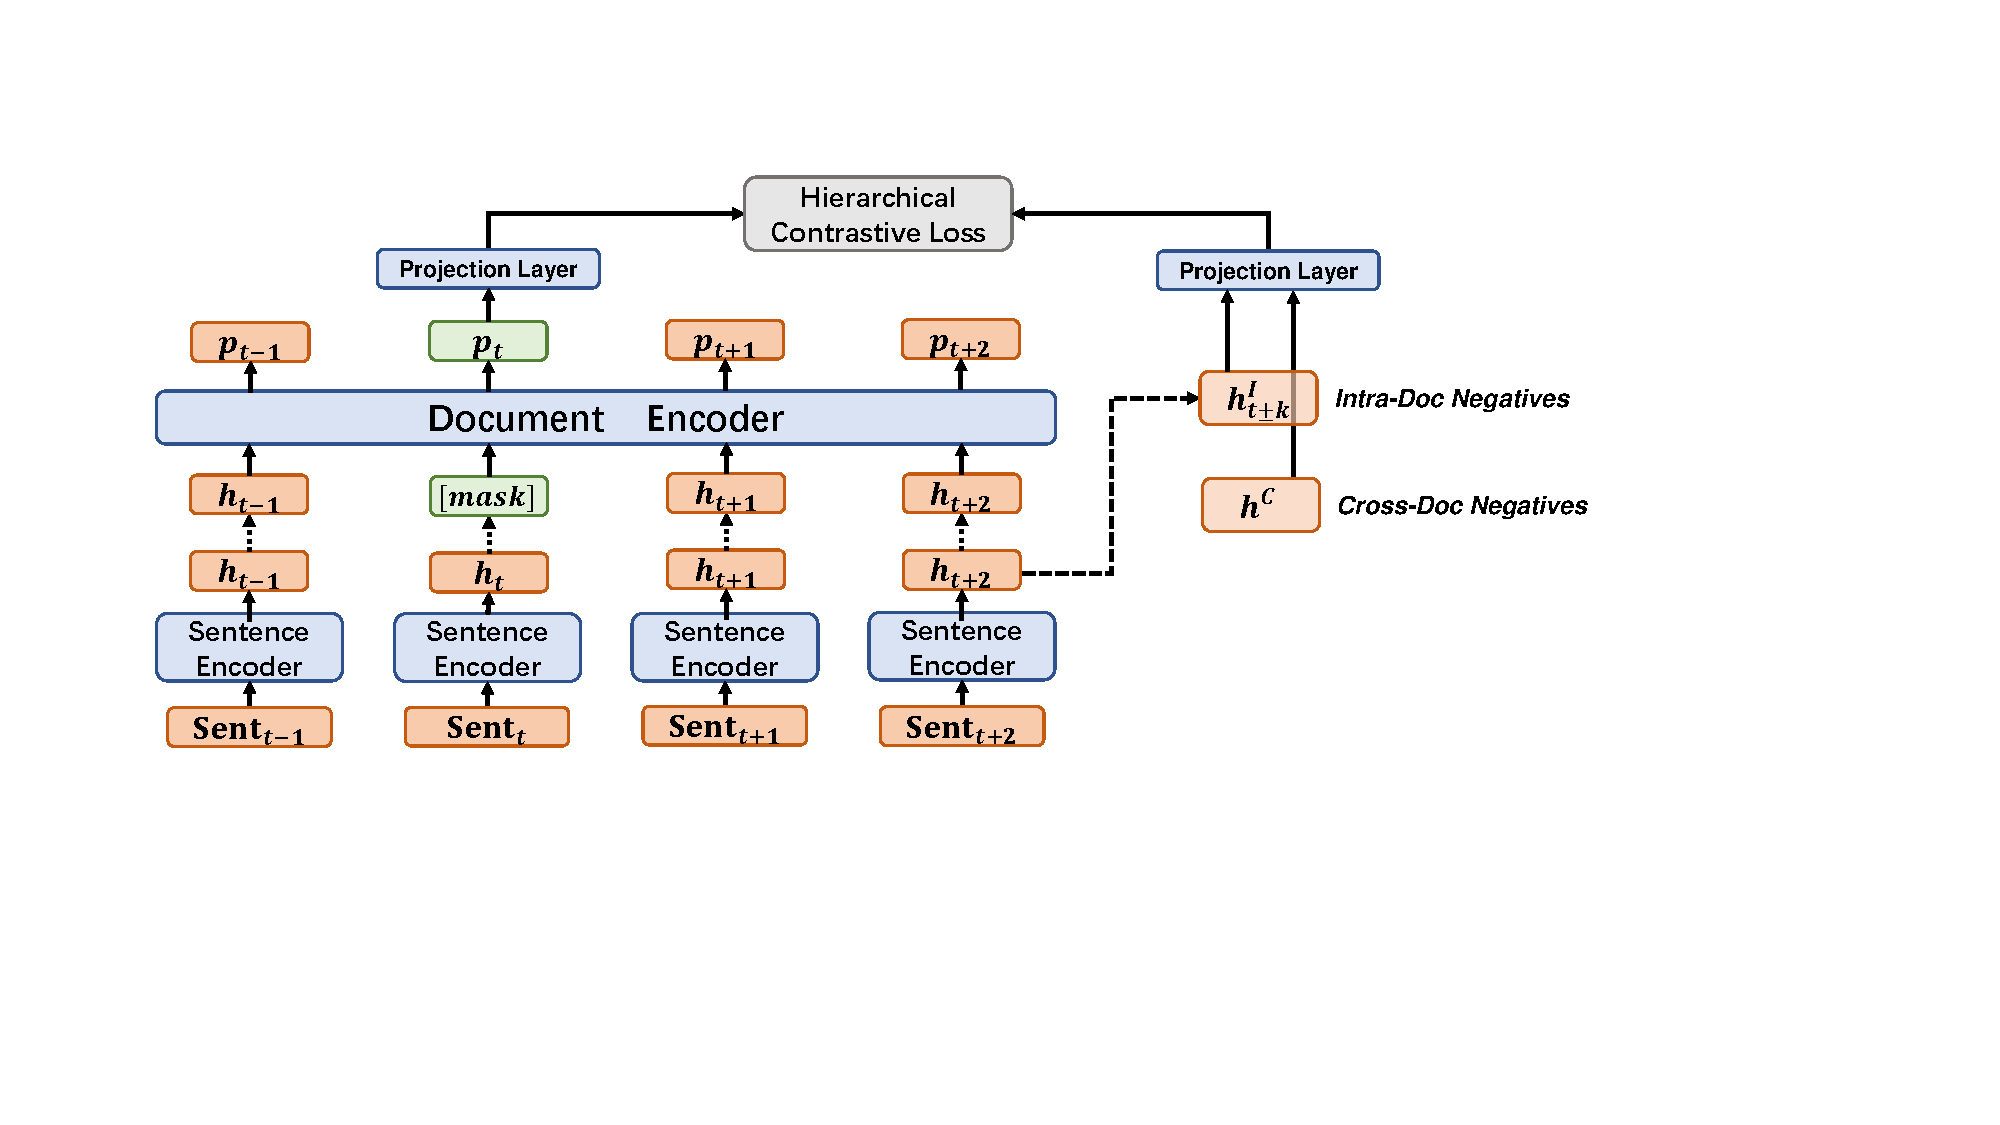
\includegraphics[width=0.9\linewidth]{pics/model.pdf}
    \caption{The general framework of masked sentence model (MSM), which has a hierarchical model architecture including the sentence encoder and the document encoder. The masked sentence prediction task predicts the masked sentence vector $p_t$, given the original vector $h_t$ as the positive anchor, via a hierarchical contrastive loss. }
    \label{fig:modelx}
\end{figure*}

% The original sentence vector $h_t$ is seen as the positive anchor for the output vector $p_t$ of document encoder corresponding to $[mask]$.

% Our Masked Sentence Encoder (MSM) to learn this universal relation and facilitate the isomorphic sentence embeddings for cross-lingual retrieval.


In this section, we first present the hierarchical model architecture. 
As illustrated in Figure.\ref{fig:modelx}, our Masked Sentence Encoder (MSM) has a hierarchical architecture that contains the Sentence Encode and the Document Encoder. The document encoder is applied to the sentence vectors generated by the sentence encoder from a sequence of sentences in a document.

\noindent{\bf Sentence Encoder. } Given a document containing a sequence of sentences ${\mathcal{D}} = (S_1,S_2,...,S_N)$ in which $S_i$ denote a sentence in document, and each sentence contains a list of words. As shown in \ref{fig:modelx}, the sentence encoder extracts the sentence representations for the sequence in a document, and the document encoder is to model the sentence relation and predict the masked sentences. First, we adopt a transformer-based encoder as our sentence encoder. Then as usual the sentence is passed through the embedding layer and transformer layers, and we take the last hidden state of the CLS token as the sentence representation. Note that all the sentence encoders share the parameters and we can get $N$ sentence vectors $\mathcal{D}_H = (h_1,h_2,...,h_N)$ respectively. In this task, we just encoder the complete sentences without the mask to get thorough sentence representations.

\noindent{\bf Document Encoder. } Then the sentence-level vectors run through the document encoder, which has similar transformer-based architecture. Considering the sentences have sequential order in a document, the sentence position is also taken into account and it doesn't have token type embedding. After equipped with sentence position embeddings, we encode them through document encoder layers to get document-level context aware embeddings $\mathcal{D}_P = (p_1,p_2,...,p_N)$. 
In order to train our model, we apply the sentence-level mask to the sentence vectors for our masked sentence prediction task. Specifically,  $\mathcal{D}_H = (h_1,h_2,...,h_N)$ are the original sentence vectors, and we mask selected sentence vector $h_t$ to $[mask]$ token and keep other the original ones. The original sentence vector $h_t$ is seen as the positive anchor for the output vector $p_t$ of document encoder corresponding to $[mask]$.
Considering a document that contains $N$ sentences, we mask each sentence in turn and keep the others the original, to get $N$ pairs of $p_t$ and $h_t$. It is effective to get as many samples as possible at the same time for efficient training. 
\textcolor{black}{Since the length of document encoder's input is not long (for the number of sentences in a document is not long) and our document encoder is also shallow, it makes our approach efficient without much computation.}

% Then the output vector $p_t$ of document encoder corresponding to $[mask]$ is seen as the positive anchor for $h_t$.

There are some models also adopting a hierarchical transformer-based model~\citep{santra-etal-2021-hierarchical}. For example, HiBERT~\citep{zhang-etal-2019-hibert} uses a multi-level transformers for document summarization, while it applies the mask to the words with a decoder for autoregressive pre-training. Poolingformer~\citep{zhang2021poolingformer} proposes a two-level pooling attention schema for long document but can't be applied for retrieval. They mainly adopt token-level MLM and targets document understanding, while ours focuses on masked sentence prediction and is directed at cross-lingual retrieval.

\subsection {Masked Sentence Prediction Task} 
\label{sec:prediction}
% Inspired by the Masked Language Model (MLM) task which reconstructs the masked token from its context of the corrupted sentences

% In order to train MSM, we adopt a sentence-level mask prediction task, which masks the selected sentence vector and predict it from the output of the document encoder.


In order to model the sentence relation, we propose a masked sentence prediction task that aligns masked sentence vectors $p_t$ with corresponding original $h_t$ via the hierarchical contrastive loss. Distinct from Masked Language Model which can directly compute cross-entropy loss between masked tokens and pre-built vocabulary, our model lacks a sentence-level vocabulary. Here we propose a novel hierarchical contrastive loss on sentence vectors to address it. Contrastive learning has been shown effective in sentence representation learning~\citep{DPR2020, gao-etal-2021-simcse}, and our model modifies the typical InfoNCE loss~\citep{oord2018representation} to a hierarchical contrastive loss for the masked sentence prediction task. As shown in Figure.\ref{fig:modelx}, for masked sentence vectors $p_t$, the positive anchor is original $h_t$ and we collect two categories of negatives: (a) Cross-Doc Negatives are the sentence vectors from different documents, i.e. $h^{\mathcal{C}}_k$, which can be seen as random negatives as usual. (b) Intra-Doc Negatives are the sentence vectors in a same document generated by sentence encoder, i.e. $h^{\mathcal{I}}_j, j{\neq}t $. Then the masked sentence vectors $p_t$ with them are passed through the projection layer, and the output vectors are involved in the hierarchical contrastive loss as: 

\begin{equation}
\label{eq:loss}
\begin{aligned}
     & \mathcal{L}_{msm}(p_t, \{h^{\mathcal{I}}_t, h^{\mathcal{I}}_1, \ldots, h^{\mathcal{I}}_{|\mathcal{I}|}, h^{\mathcal{C}}_1, \ldots, h^{\mathcal{C}}_{|\mathcal{C}|}\}) 
    \\ = & -\log \frac{e^{\operatorname{sim}\left(p_{t}, h^{\mathcal{I}}_t\right)}}{{e^{\operatorname{sim}\left(p_{t}, h^{\mathcal{I}}_t\right) - }+\sum_{j=1, j{\neq}t}^{|\mathcal{I}|} e^{\operatorname{sim}\left(p_{t}, h^{\mathcal{I}}_j\right) - \mu{\alpha}}}{+ \sum_{k=1}^{|\mathcal{C}|} e^{\operatorname{sim}\left(p_{t}, h^{\mathcal{C}}_k\right)}}}
\end{aligned}
\end{equation}

% where $h^{\mathcal{I}}_j, j{\neq}t $ indicates the intra-doc negatives, and $h^{\mathcal{C}}_k$ indicates the cross-doc negatives.

In the previous study~\citep{gao2021cocondenser}, two sampled views or sentences of the same document are often seen as a positive pair to leverage their correlation. However, it limits the representation capability for it encourages the alignment between two views, just as a coarse-grained topic model~\citep{yan2013biterm}. In contrast, we treat them as Intra-Doc Negatives, which could help the model to distinguish sentences from the same document to learn fine-grained representations. The intra-doc samples usually have closer semantic relation than cross-doc ones and directly treating them as negatives could hurt the uniformity of embedding space. To prevent this negative impact, we set the dynamic bias subtracted from their similarity scores. As seen in Eq.\ref{eq:loss}, the dynamic bias is $-{\mu}{\alpha}$ in which $\mu$ is a hyper-parameter and $\alpha$ is computed as:


\begin{small} 
\begin{equation}
\label{eq:bias}
\begin{aligned}
     {\alpha} = & \left(\frac{\sum_{j=1, j{\neq}t}^{|\mathcal{I}|} \operatorname{sim}\left(p_{t}, h^{\mathcal{I}}_j\right)} {|\mathcal{I}| - 1} 
     - \frac{\sum_{k=1}^{|\mathcal{C}|} \operatorname{sim}\left(p_{t}, h^{\mathcal{C}}_k\right)}{|\mathcal{C}|} \right).detach()
\end{aligned}
\end{equation}
\end{small}


\noindent It represents the gap between the average similarity score of Intra-Doc Negatives and them from Cross-Doc Negatives. Subtracting the dynamic bias can tune the high similarity of intra-doc negatives to the level of cross-doc negatives, which can also be seen as interpolation to generate soft samples. Note that we only use the value but do not pass the gradient, so we adopt the detach function after computation. Our experimental result in Sec.\ref{sec:analysis} validates that the hierarchical contrastive loss is beneficial for representation learning in our model.


% We provide more mathematical details in Appendix.\ref{ap:math} and our experimental result in Sec.\ref{sec:analysis} validate the hierarchical contrastive loss is beneficial.


% 把同一个document的当做正例,判定同一topic,退化成topic-model,粗粒度的句子关系。
% 同一个document的句子,会产生相同embedding
% 但是他们相似度仅次于原始句子,INFONCE会把他们train到一起,所以需要一些分层的设计


Considering the expensive cost of pre-training from scratch, we initialize the sentence encoder with pre-trained XLM-R weight and solely the document encoder from scratch. 
To prevent gradient back propagated from the randomly initialized document encoder from damaging sentence encoder weight, we adopt MLM task to impose a semantic constraint. Therefore our total loss consists of a token-level MLM loss and a sentence-level contrastive loss:


\begin{equation}
\label{eq:all}
\begin{aligned}
     & \mathcal{L} = \mathcal{L}_{msm} + \mathcal{L}_{mlm}
\end{aligned}
\end{equation}

% where the MLM is applied on the sentence encoder in a multi-task schema. 
% which provides a fair comparison to the original pre-trained model. 

After pre-training, we discard the document encoder and leave the sentence encoder for fine-tuning. \textcolor{black}{
In fact, the document encoder in our MSM plays as a bottleneck~\citep{li-etal-2020-optimus}: the sentence encoder press the sentence semantics into sentence vectors, and the document encoder leverage the limited information to predict the masked sentence vector, thus enforcing an information bottleneck on the sentence encoder for better representations. It also coincides with the recent works utilizing similar bottleneck theory for better text encoders~\citep{lu-etal-2021-less, liu2022retromae}. By the way, the sentence encoder has the same architecture as XLMR, which ensures a fair comparison. 
}

% As we have stated in Sec.\ref{subsec:dr}, there are several methods generating two mutually exclusive views of a document for contrastive pre-training, including ICT~\citep{lee-etal-2019-latent} and CROP~\citep{gao2021cocondenser}. 
% Compared to them, ours is a more general way to utilize sequential relations and can learn shared sentence relations across languages.

% In addition, there are some explorers utilizing auto-encoders bottleneck to pre-train a better encoder for dense retrieval. Our MSM also coincides with its idea to some extent: the sentence encoder press the sentence semantics into CLS and the document encoder leverage the limited information to reconstruct the masked sentence vector. 




\vspace{-0.2cm}
\section{Experiment}\label{sec:exp}
\vspace{-0.2cm}
In this section, we present the experimental results to validate the effectiveness of the proposed BAT algorithm on benchmark datasets and compare it with state-of-the-art baseline methods. We also verify that both two components are helpful and necessary for BAT. The implementation of the BAT can be found via \url{https://anonymous.4open.science/r/benign-adv-77C5}.

\vspace{-0.2cm}
\subsection{Experimental Setup}
\vspace{-0.1cm}
%\jt{we can put baselines here.} \\
%\jt{implementation details, such as optimization method}
In this work, in order to demonstrate the 
merit of BAT, we conduct the experiments mainly on benchmark datasets CIFAR100~\cite{krizhevsky2009learning} and Tiny~ImageNet~\cite{le2015tiny}, which are relatively complex datasets (i.e., containing larger fractions of atypical samples). For both datasets, we study the algorithms under the model architectures ResNet and WideResNet (WRN)~\cite{he2016deep}. In this section, we only present the results of ResNet18 for CIFAR100 and ResNet32 for Tiny~ImageNet and leave the results on WRN in Appendix~\ref{app:exp}. As a fair comparison with BAT, we implement the baseline algorithms including PGD adversarial training~\cite{madry2017towards} as well as its most popular variant TRADES~\cite{zhang2019theoretically}. In addition, we include several recent algorithms: MART~\cite{wang2019improving} and GAIRAT~\cite{zhang2020geometry}, which also incorporate reweighting strategies into adversarial training. For BAT and all baseline methods, we run the algorithms using SGD~\cite{bottou2010large} for 160 epochs with the learning rate that starts from 0.1 and decays by 0.1 after the epoch 80 and 120. More implementation details can be found in Appendix~\ref{app:exp}.

\textbf{Performance on CIFAR100.} For a comprehensive comparison between different methods on CIFAR100, in the results from Table~\ref{Tab:results_cifar100}, we report the models' clean accuracy and adversarial accuracy against $l_\infty$-$8/255$ PGD attack~\cite{madry2017towards}, as well as their performance on the typical sample set and atypical sample set (as described in Section~\ref{sec:pre}). A more comprehensive robustness evaluation on different attacking methods (including CW~\cite{carlini2017towards} and Auto-Attack~\cite{croce2020reliable}) are presented in Appendix~\ref{app:exp}. For BAT, we report its performance when choosing its optimal hyperparameter: $\alpha = 1  ~\text{\&} ~2$ and $\beta = 0.2$. In the Section~\ref{sec:ablation}, we will discuss the impact of the selection of $\alpha$ and $\beta$ on BAT. For baseline methods, the settings and checkpoint selections follow the original papers' suggestions.

%Note that the main goal of BAT is not to improve model's adversarial robustness, so we leave the robustness evaluation with additional attacking methods, such as CW~\cite{carlini2017towards} and Auto Attack~\cite{croce2020reliable} in  Appendix~\ref{app:exp} where we have similar observations.

\vspace{-0.3cm}
\begin{table}[h]
\small
\centering
\caption{Performance of BAT vs. Baselines on CIFAR100 Under ResNet18}
\begin{tabular}{c|cc|cc|cc}
\hline
Method & All Acc. & All Adv. & Typical Acc. & Typical Adv. & Atyp. Acc. & Atyp. Adv. \\
\hline
\hline
PGD Train (Best Adv.) & 56.9 & 27.4 & 90.6 & 59.0 &29.5 & 7.7\\
PGD Train (Best Clean) & 57.8 & 21.9 & 88.3 & 51.0 & \textbf{40.1} & 8.3 \\
%TRADES ($1/\lambda = 1$) & \textbf{61.3} & 21.9 & \textbf{93.0} & 50.0 & 44.7 & 7.9\\
TRADES ($1/\lambda = 5$) & 56.6 & 26.9 & 88.9 & 57.1 & 37.3 & \textbf{10.9} \\
MART~\cite{wang2019improving} & 51.8 & \textbf{30.4} & 85.3 & \textbf{62.2} & 25.3 & 10.1\\
GAIRAT~\cite{zhang2020geometry} & 58.2 & 27.8 & 90.6 & 60.7 & 31.6 & 8.2\\
\hline
BAT ($\alpha = 1, \beta = 0.2$) & \textbf{59.5} &27.3 & \textbf{92.3} & 58.8 & 36.3 & 8.7 \\
BAT ($\alpha = 2, \beta = 0.2$) &59.3 & 27.4 & \textbf{92.3} & 60.3 & 33.1 & 7.4 \\
\hline
\hline
\end{tabular}
\label{Tab:results_cifar100}
\end{table}
\vspace{-0.2cm}
From the results in Table~\ref{Tab:results_cifar100}, we can find that BATs enjoy good clean \& adversarial accuracy trade-off among all methods. It is because BATs can obtain the highest overall clean accuracy ($\sim59.5\%$), as well as comparably good adversarial accuracy ($\sim27.3$) with baseline methods. The only exception is MART~\cite{wang2019improving} which has the higher adversarial accuracy around $\sim 30\%$. However, MART~\cite{wang2019improving} has much lower clean accuracy than BATs. 

To gain a deeper understanding of the working mechanism of BAT, we focus on the performance on BAT vs. PGD adversarial training~\cite{madry2017towards}. Compared with PGD adversarial training with highest adversarial accuracy (PGD Train (Best Adv.)), the BAT methods are $2\sim3\%$ higher in terms of overall clean accuracy, and similar adversarial accuracy. The improvement of clean accuracy is mainly due to BATs' capacity to fit much more atypical samples. For example, the clean accuracy of BAT ($\alpha=1, \beta=0.2$) is about $6\%$ higher than PGD Train~(Best Adv.). On the other hand, compared to PGD adversarial training with the highest clean accuracy (PGD Train (Best Clean)), BATs have much better overall adversarial robustness and slightly better clean accuracy. This is mainly due to BAT's advantage on typical samples, because BATs can successfully prevent the performance drop of typical samples during the training process. Since BATs can achieve good performance on both typical samples and atypical samples, BATs outperform PGD adversarial training in CIFAR100.

\begin{wrapfigure}{r}{0.6\textwidth}
\vspace{-0.4cm}
\subfloat{
\begin{minipage}[c]{0.3\textwidth}
\centering
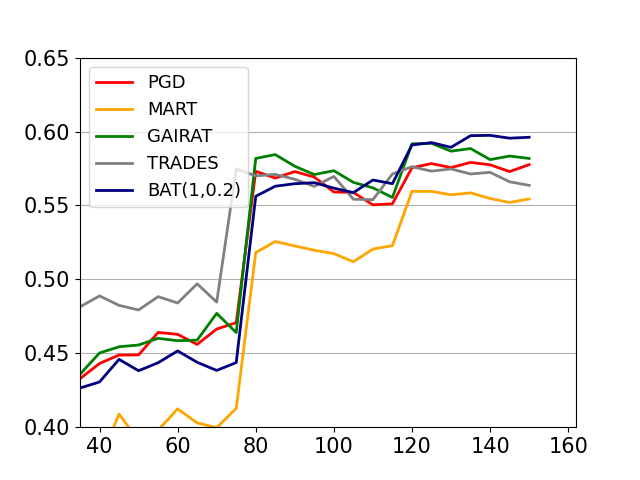
\includegraphics[width = 1.1\textwidth]{figures/base_clean.png}
\end{minipage}
}
\subfloat{
\begin{minipage}[c]{0.3\textwidth}
\centering
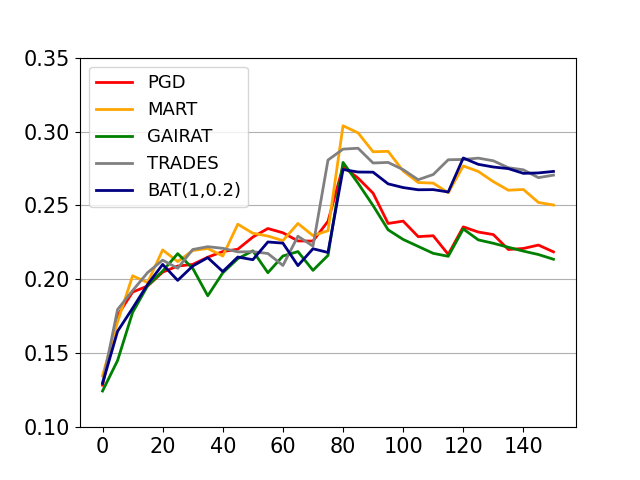
\includegraphics[width = 1.1\textwidth]{figures/base_rob.png}
\end{minipage}
}
\vspace{-0.4cm}
\caption{\small Clean Acc. (left) \& Adv. Acc (right)}
\label{fig:exp1}
\end{wrapfigure}
In Fig.~\ref{fig:exp1}, we also show the change of each models' overall clean accuracy (Fig~\ref{fig:exp1} (left)) \& adversarial accuracy (Fig~\ref{fig:exp1} (right)) along with the training progress. 
Interestingly, similar to PGD adversarial training, all baseline methods cannot achieve the optimal clean and adversarial accuracy at the same moment.
They always achieve the best adversarial accuracy around Epoch 80 (right after the first time weight decay), and the best clean accuracy on the last epochs. However, for BATs, since they can effectively prevent the robustness dropping in the late epochs, BATs are able to train until last epochs and enjoy good clean and adversarial accuracy simultaneously.
%As a result, BATs have higher clean accuracy than all baseline models, and good adversarial accuracy, which are similar or comparable to all baselines (even on their best checkpoints).

\textbf{Performance on Tiny~ImageNet.} Tiny~ImageNet~\cite{le2015tiny} contains 200 classes of the images in the original ImageNet~\cite{krizhevsky2012imagenet} dataset, with 500 training images for each class, and image size $64\times 64$. In our experiments, we only choose the first 50 classes in Tiny ImageNet for training and prediction. Since the image size is $64\times 64$, for both training and robustness evaluation, we consider the adversarial attacks are bounded by $l_\infty$-norm-4/255. In Table~\ref{Tab:results_imagenet}, we report the performance of BAT and baseline methods. Similar to the conclusions we can make from CIFAR100, BATs can achieve the highest overall clean accuracy and comparably good adversarial accuracy with baseline methods. 
\begin{table}[h]
\small
\vspace{-0.2cm}
\centering
\caption{Performance of BAT vs. Baselines on Tiny~ImageNet Under ResNet32}
\begin{tabular}{c|cc|cc|cc}
\hline
Method & All Acc. & All Adv. & Typical Acc. & Typical Adv. & Atyp. Acc. & Atyp. Adv. \\
\hline
\hline
Adv. Train (Best Adv.) & 56.3 & 32.3 & 97.5 & 85.3 &41.5 & 9.6\\
Adv. Train (Best Clean) & 58.2 & 30.5 & 98.0 & 80.4 & 44.7 & 9.1 \\
TRADES ($1/\lambda = 5$) & 55.4 & 28.8 & 97.3 & 77.4 & 38.8 & 9.6 \\
MART~\cite{wang2019improving} & 56.2 & \textbf{34.5} & 97.7 & 85.1 & 41.4 & \textbf{13.6} \\
GAIRAT~\cite{zhang2020geometry} & 58.4 & 30.4 & 98.0 & 81.7 & 45.7 & 7.8\\
\hline
BAT ($\alpha = 1, \beta = 0.2$) & \textbf{59.4} &32.0 & 98.4 & 83.9 & \textbf{48.4} & 10.2 \\
BAT ($\alpha = 2, \beta = 0.2$) &\textbf{59.4} &32.9 & \textbf{99.1} & \textbf{86.9} & 45.7 & 10.9 \\
\hline
\hline
\end{tabular}
\label{Tab:results_imagenet}
\end{table}

\vspace{-0.7cm}
\subsection{Ablation Study}\label{sec:ablation}
\vspace{-0.2cm}
\begin{wrapfigure}{r}{0.6\textwidth}
\vspace{-0.9cm}
\subfloat{
\begin{minipage}[c]{0.32\textwidth}
\centering
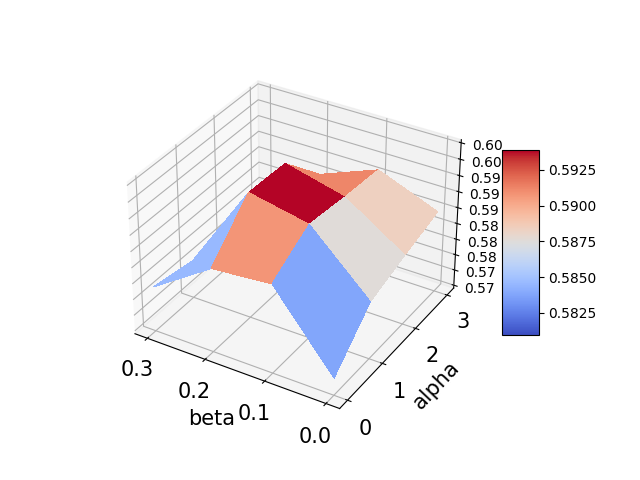
\includegraphics[width = 1.1\textwidth]{figures/abl_clean.png}
\end{minipage}
}
\subfloat{
\begin{minipage}[c]{0.32\textwidth}
\centering
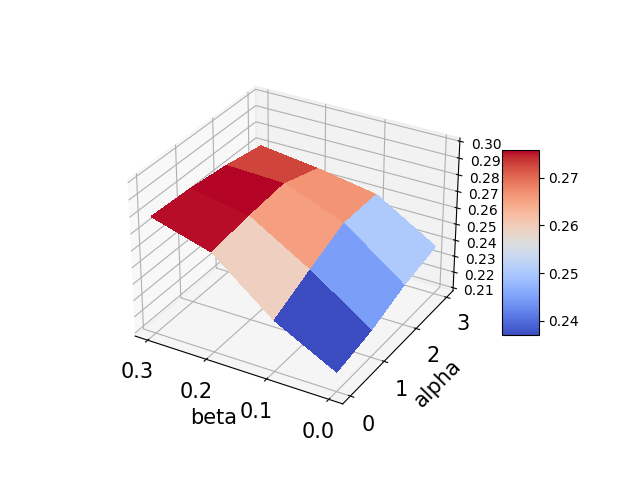
\includegraphics[width = 1.1\textwidth]{figures/abl_rob.png}
\end{minipage}
}
\caption{\small Clean Acc.(left) \& Adv. Acc.(right)}
\label{fig:exp2}
\vspace{-0.2cm}
\end{wrapfigure}
In this subsection, we study the potential impact of the hyperparameters chosen in BAT, which is $\alpha$ that controls the \textit{Reweighting} process and $\beta$ that controls the \textit{Discrimination Loss}. 
In Fig.~\ref{fig:exp2}, we conduct the experiments on CIFAR100 with BAT when $\alpha$ is chosen in [0,1,2,3] and $\beta$ is in [0, 0.1, 0.2, 0.3].
In Fig.~\ref{fig:exp2}, we show each model's overall clean accuracy~(left) \& adversarial accuracy~(right) along the Z-axis, and X-axis / Y-axis indicate the models' corresponding variables of $(\alpha,\beta)$. Note that when $\alpha=\beta=0$, the BAT method regresses to original PGD adversarial training. From the result, we can see that a positive pair of $(\alpha,\beta)$ can benefit both model clean and adversarial accuracy. Therefore, both two components \textit{Reweighting} and \textit{Discrimination Loss} of BAT are helpful and necessary. However, when $\alpha$ or $\beta$ is relatively too large, it will hurt the BAT's clean accuracy. As a result, in CIFAR~100, when $\alpha=1$ or 2 and $\beta= 0.2$, BAT can achieve the optimal performance.

%If we look at the performance of these models at their final epochs, we first observe that $\beta=0.2$ can improve both clean and adversarial accuracy, compared to all models with $\beta = 0$. Moreover, given any fixed value of $\beta$, the model with $\alpha = 1$ or 2 always outperforms than $\alpha=0$.
%Since a positive $\alpha$ indicates the BAT algorithm downweight or exclude certain samples during the training process, we can conclude that those  samples which are downweighted/excluded are acting like poisoning samples to deteriorate the models' performance. and necessary.



\section{Conclusion}
In this paper, we propose a novel masked sentence model which leverages sequential sentence relation for pre-training to improve cross-lingual retrieval. It contains a two-level encoder in which the document encoder applied to the sentence vectors generated by the sentence encoder from a sequence of sentences. Then we propose a masked sentence prediction task to train the model, which masks and predicts the selected sentence vector via a hierarchical contrastive loss with sampled negatives. Through comprehensive experiments on 4 cross-lingual retrieval benchmark datasets, we demonstrate that MSM significantly outperforms existing advanced pre-training methods. Our further analysis and detailed ablation study clearly show the effectiveness and stronger cross-lingual retrieval capabilities of our approach. Code and model will be made publicly available.

% Starting from an observation that sequential sentence relation are universal across languages, we propose a multilingual PLM leveraging it to improve cross-lingual retrieval, called masked sentence model (MSM). It consists of a sentence encoder to generate the sentence representations, and a document encoder applied to a sequence of sentence vectors from a document. The document encoder is shared for all languages to model the universal sequential sentence relation across languages. To predict the masked sentence in MSM task, we propose a hierarchical contrastive loss with sampled negatives. Comprehensive experiments on four cross-lingual retrieval tasks show MSM significantly outperforms existing advanced pre-training models, demonstrating the effectiveness and stronger cross-lingual retrieval capabilities of our approach.

% \subsubsection*{Acknowledgments}
% Use unnumbered third level headings for the acknowledgments. All
% acknowledgments, including those to funding agencies, go at the end of the paper.

% \bibliography{iclr2023_conference, anthology}
\bibliography{iclr2023_conference}
\bibliographystyle{iclr2023_conference}

\appendix


% \setcounter{lemma}{0}
%     \renewcommand{\thelemma}{\Alph{section}\arabic{lemma}}
    
\begin{comment}
\end{comment}

{\colorred 
\section{Compatible Value Function}
\label{app:comp_v}

The original policy gradient with compatible value function is stated as follow. 
\begin{theorem}
[\cite{sutton1999policy}]
Let $Q_w$ be a state-action function with parameter $w$ and $\pi_\theta$ be a policy function with parameter $\theta$. 
If $Q_w$ satisfies $\mathbb{E}_{\pi} [(Q^\pi - Q_w) \nabla_w Q_w] = 0$ and 
$\nabla_w Q_w = \nabla_\theta \log \pi_\theta,$
then $$\nabla_\theta \mathcal{J} = \mathbb{E}_\pi [Q_w \nabla_\theta \log \pi_\theta].$$
\label{thm:pg_fa}
\end{theorem}
If we let $w = \theta$ in Theorem \ref{thm:pg_fa}, where $Q_w$ and $\pi_\theta$ share parameters, we have the following theorem. 
\begin{theorem}
Let $Q_\theta$ be a state-action function with parameter $\theta$ and $\pi_\theta$ be a policy function with parameter $\theta$. 
If $Q_\theta$ satisfies $\mathbb{E}_{\pi} [(Q^\pi - Q_\theta) \nabla_\theta Q_\theta] = 0$ and 
$\nabla_\theta Q_\theta = \nabla_\theta \log \pi_\theta,$
then $$\nabla_\theta \mathcal{J} = \mathbb{E}_\pi [Q_\theta \nabla_\theta \log \pi_\theta].$$
\label{thm:pg_fa2}
\end{theorem}
Define 
$$\chi \overset{def}{=} \mathbb{E}_\pi [\cos <\nabla_\theta Q_\theta, \nabla_\theta \log \pi_\theta>].$$
We show that $\chi = 1$ is the necessary condition for the compatible condition $\nabla_\theta Q_\theta = \nabla_\theta \log \pi_\theta$. 
\begin{theorem}
i) If $\nabla_\theta Q_\theta \propto \nabla_\theta \log \pi_\theta$ for all states, then $\chi = 1$.

ii) If $\chi = 1$, then $\nabla_\theta Q_\theta \propto \nabla_\theta \log \pi_\theta$ for all states. 
\label{thm:connect_cond}
\end{theorem}
By Theorem \ref{thm:connect_cond}, $\chi = 1$ is equivalent to $\nabla_\theta Q_\theta \propto \nabla_\theta \log \pi_\theta$, and $\nabla_\theta Q_\theta \propto \nabla_\theta \log \pi_\theta$ is the necessary condition for $\nabla_\theta Q_\theta = \nabla_\theta \log \pi_\theta$, hence $\chi = 1$ is the necessary condition for $\nabla_\theta Q_\theta = \nabla_\theta \log \pi_\theta$.
\begin{proof}
i) Since $\nabla_\theta Q_\theta \propto \nabla_\theta \log \pi_\theta$, we have $<\nabla_\theta Q_\theta, \nabla_\theta \log \pi_\theta> = 0$. 
By definition of $\chi$, we have 
$$\chi = \mathbb{E}_\pi [\cos <\nabla_\theta Q_\theta, \nabla_\theta \log \pi_\theta>] = \mathbb{E}_\pi [1] = 1.$$

ii) Since $\chi \leq 1$ and $\cos(x)$ is monotonic decreasing as $x$ goes from $0$ to $\pi$, the equality $\chi = 1$ only holds when all states satisfy $\cos <\nabla_\theta Q_\theta, \nabla_\theta \log \pi_\theta> = 0$, which means $\nabla_\theta Q_\theta \propto \nabla_\theta \log \pi_\theta$. 
\end{proof}
}

% $$
% \begin{aligned}
%     logp &= variable((3, 3, 4)) \\
%     q &= variable((3, 3, 4)) \\
%     alpha &= 0.3 \\
%     \pi &= softmax(alpha * logp + (1.0 - alpha) * q) \\
% \end{aligned}
% $$
\clearpage

\section{Gradients Between Policy Improvement and Policy Evaluation}
\label{app:mtv}

\begin{table}[hb!]
    \centering
    \scalebox{0.90}{
    \begin{math}
        \begin{array}{c|c|c|c}
    \toprule
     & \text{Function Approximation} & \text{Train Gradients} & \text{Cosine of Interested Angles} \\
    \midrule
    
    \text{PPO} & (V, logit) = (V_\theta, logit_\theta) & 0.5 \nabla L_V + \nabla \mathcal{J} & %\cos<\nabla L_V, \nabla \mathcal{J}> 
    \\ 
    & \pi = \text{softmax}(logit) & & \\
    
    \midrule
    
    \text{PPO ver.1} & (Q, logit) = (Q_\theta, logit_\theta), & 0.5 \nabla L_V + \nabla \mathcal{J} & \cos<\nabla L_Q, \nabla \mathcal{J}>%\cos<\nabla L_V, \nabla \mathcal{J}> 
    \\
    & \pi = \text{softmax}(logit) & & \cos<\nabla Q, \nabla \log \pi> \\
    & V = sg(\pi)\cdot Q & & %\cos<\nabla L_V, \nabla L_Q> 
    \\
    % & & &  \\
    
    \midrule
    
    \text{PPO ver.2} & (Q, logit) = (Q_\theta, logit_\theta), & 0.5 \nabla L_V + \nabla L_Q + \nabla \mathcal{J} & \cos<\nabla L_Q, \nabla \mathcal{J}> %\cos<\nabla L_V, \nabla \mathcal{J}> 
    \\
    & pi = \text{softmax}(logit) & & \cos<\nabla Q, \nabla \log \pi> \\
    & V = sg(\pi)\cdot Q & & %\cos<\nabla L_V, \nabla L_Q> 
    \\
    % & & &  \\
    
    \midrule
    
    \text{PPO+CASA} & (V, A) = (V_\theta, A_\theta), & 0.5 \nabla L_V + \nabla L_Q + \nabla \mathcal{J} & \cos<\nabla L_Q, \nabla \mathcal{J}> %\cos<\nabla L_V, \nabla \mathcal{J}> 
    \\
    & \pi = \text{softmax}(A/\tau), & & \cos<\nabla Q, \nabla \log \pi> \\
    & \Bar{A} = A - sg(\pi) \cdot A & & %\cos<\nabla L_V, \nabla L_Q> 
    \\
    & Q = \Bar{A} + sg(V) & &  \\
    
    \bottomrule 
    \end{array}
    \end{math}
    }
    
    \caption{PPO is the original PPO. PPO ver.1 and PPO ver.2 are adapted versions to calculate $\nabla L_Q$. PPO+CASA is applying CASA on PPO, which is described in Sec. \ref{sec:on_ppo_and_r2d2}.}
    \label{tab:ppo_mtv}
\end{table}

\begin{table}[ht!]
    \centering
    \scalebox{0.90}{
    \begin{math}
        \begin{array}{c|c|c|c}
    \toprule
     & \text{Function Approximation} & \text{Train Gradients} & \text{Cosine of Interested Angles} \\
    \midrule
    
    \text{R2D2} & (V, A) = (V_\theta, A_\theta) & \nabla L_Q & \cos<\nabla L_Q, \nabla \mathcal{J}>  %\cos<\nabla L_V, \nabla \mathcal{J}> 
    \\
    & Q = A + V & & \\
    & \pi = \text{softmax}(A / \tau) & & %\cos<\nabla L_V, \nabla L_Q> 
    \\
    % & & &  \\ % <\nabla Q, \nabla \log \pi>

    \midrule
    
    \text{R2D2 ver.1} & (V, A) = (V_\theta, A_\theta) & 0.5 \nabla L_V + \nabla L_Q & \cos<\nabla L_Q, \nabla \mathcal{J}>  % \cos<\nabla L_V, \nabla \mathcal{J}> 
    \\
    & Q = A + V & & % \cos<\nabla L_Q, \nabla \mathcal{J}> 
    \\
    & \pi = \text{softmax}(A / \tau) & & % \cos<\nabla L_V, \nabla L_Q> 
    \\
    % & & &  \\ % \cos<\nabla Q, \nabla \log \pi>

    \midrule
    
    \text{R2D2+CASA} & (V, A) = (V_\theta, A_\theta), & 0.5 \nabla L_V + \nabla L_Q + \nabla \mathcal{J} & \cos<\nabla L_Q, \nabla \mathcal{J}>  % \cos<\nabla L_V, \nabla \mathcal{J}> 
    \\
    & \pi = \text{softmax}(A/\tau),  & & %\cos<\nabla L_Q, \nabla \mathcal{J}> 
    \\
    & \Bar{A} = A - sg(\pi) \cdot A & & % \cos<\nabla L_V, \nabla L_Q> 
    \\
    & Q = \Bar{A} + sg(V) & &  \\ %\cos<\nabla Q, \nabla \log \pi>
    \bottomrule 
    \end{array}
    \end{math}
     }
    \caption{R2D2 is the original R2D2. R2D2 ver.1 is adapted version to include $\nabla L_V$ for training. R2D2+CASA is applying CASA on R2D2, which is described in Sec. \ref{sec:on_ppo_and_r2d2}.}
    \label{tab:r2d2_mtv}
\end{table}

To understand the behavior of 
{\colorred $$
    \beta \overset{def}{=} <\mathbb{E}_\pi[(Q^\pi-Q_\theta)\nabla_\theta Q_\theta],\, \mathbb{E}_\pi[(Q^\pi-V_\theta) \nabla_\theta \log \pi_\theta]>
$$
}
and 
{\colorred 
$$\chi \overset{def}{=} \mathbb{E}_\pi [\cos <\nabla_\theta Q_\theta, \nabla_\theta \log \pi_\theta>]$$
}
in reinforcement learning algorithms, we choose PPO as a representative for policy-based methods and R2D2 as a representative for value-based algorithms. 

Define $$L_V(\theta) = \mathbb{E}_\pi [ (V^{\pi} - V_\theta)^2 ],\  L_Q(\theta) = \mathbb{E}_\pi [ (Q^{\pi} - Q_\theta)^2 ],$$
and $$\nabla_\theta \mathcal{J}(\theta) = \mathbb{E}_\pi \left[ (Q^{\pi}  - V_\theta ) \nabla_\theta \log \pi \right].$$
We usually have above three kinds of loss functions in reinforcement learning, which aim to estimate the state values, state-action values and the policy. 
We do not talk about the estimations of $V^\pi$ and $Q^\pi$ as they are estimated as their usual way of PPO's and R2D2's. 
All hyperparameters are listed in Appendix \ref{app:hyperparameters}. 

{\colorred For brevity, we write 
$$\cos<\nabla Q, \nabla \log \pi> = \mathbb{E}_\pi [\cos <\nabla_\theta Q_\theta, \nabla_\theta \log \pi_\theta>],$$
and
$$
\begin{aligned}
    &\cos<\nabla L_Q, \nabla \mathcal{J}> = \cos<\mathbb{E}_\pi[(Q^\pi-Q_\theta)\nabla_\theta Q_\theta],\, \mathbb{E}_\pi[(Q^\pi-V_\theta) \nabla_\theta \log \pi_\theta]>, \\
    &\cos<\nabla L_V, \nabla \mathcal{J}> = \cos<\mathbb{E}_\pi[(V^\pi-V_\theta)\nabla_\theta V_\theta],\, \mathbb{E}_\pi[(Q^\pi-V_\theta) \nabla_\theta \log \pi_\theta]>, \\
    &\cos<\nabla L_V, \nabla L_Q> = \cos<\mathbb{E}_\pi[(V^\pi-V_\theta)\nabla_\theta V_\theta],\, \mathbb{E}_\pi[(Q^\pi-Q_\theta) \nabla_\theta Q_\theta]>. \\
\end{aligned}
$$}

The fact that PPO only has $\nabla_\theta L_V$ and $\nabla_\theta \mathcal{J}$ and R2D2 only has $\nabla_\theta L_Q$ is the main difficulty to track $\cos(\beta)$ and $\chi$. 
To solve the problem, we adjust PPO and R2D2 with different versions.

For PPO, we displace the estimation of $V_\theta$ by $sg(\pi)\cdot Q_\theta$, where $Q_\theta$ is estimated by function approximation and $V_\theta$ is estimated by taking the expectation of $Q_\theta$.
All versions of PPO are listed in Table \ref{tab:ppo_mtv}.

For R2D2, we point out that though we apply $\epsilon$-greedy to interact with environments, $\epsilon$ is only used for exploration and the final target policy of value-based methods is simply $\arg\max Q_\theta$. 
Because $\arg\max Q_\theta$ breaks the gradient, we use a surrogate policy to approximate the gradient of policy improvement. 
% \haosen{potential context, the necessity of measuring the policy gradient and ``entropy'' of the Q function is that R2D2's greedy policy changes rapidly, and the rapid change give R2D2 the implicit exploration ability. \citep{policychurn} }
Since R2D2 uses dueling structure and $\text{softmax}(A_\theta / \tau) = \text{softmax}(Q_\theta / \tau) \overset{\tau \rightarrow 0+}{\longrightarrow} \arg\max Q_\theta$, we use $\pi_{surrogate} = \text{softmax}(A_\theta / \tau)$ to calculate the policy gradient. 
We only use $\pi_{surrogate}$ on learner to calculate the gradient, where the policy that interacts with environments is still $\epsilon$-greedy. 
All versions of R2D2 are listed in Table \ref{tab:r2d2_mtv}.

% Results are shown in Figure \ref{fig:mtv_app}.


% \begin{figure}[hb!]
% % \centering
% 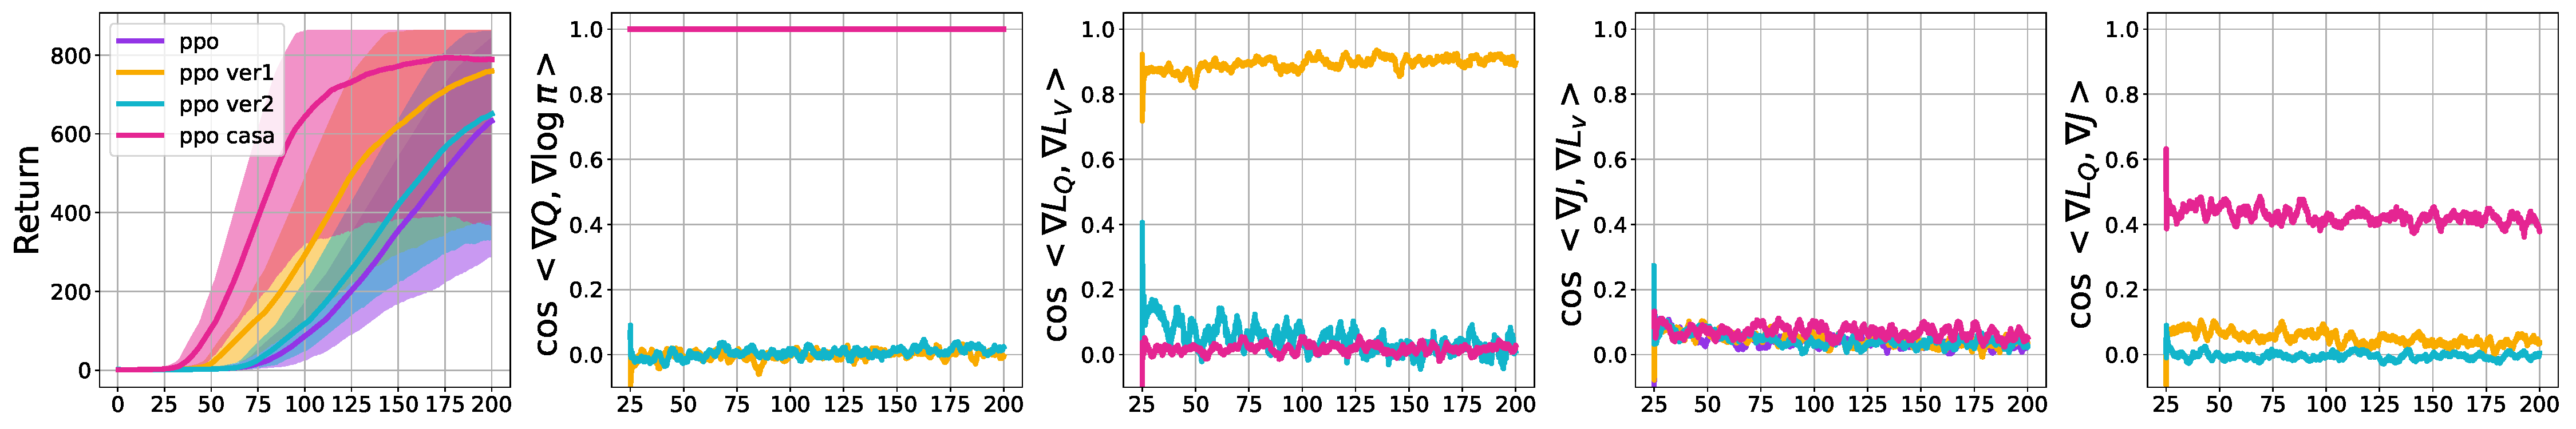
\includegraphics[width=\linewidth]{body/app_fig/app_ppo_Breakout.pdf}

% 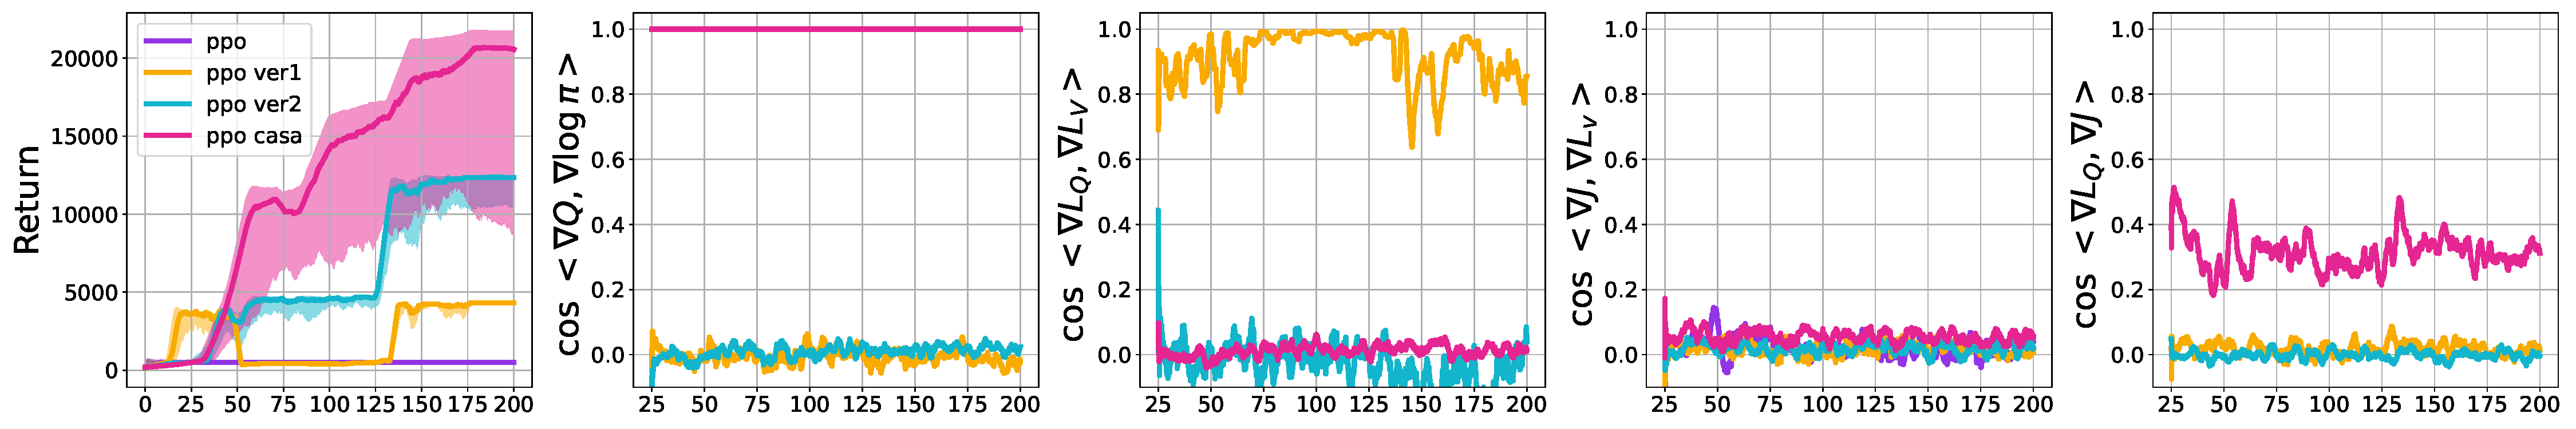
\includegraphics[width=\linewidth]{body/app_fig/app_ppo_Qbert.pdf}

% 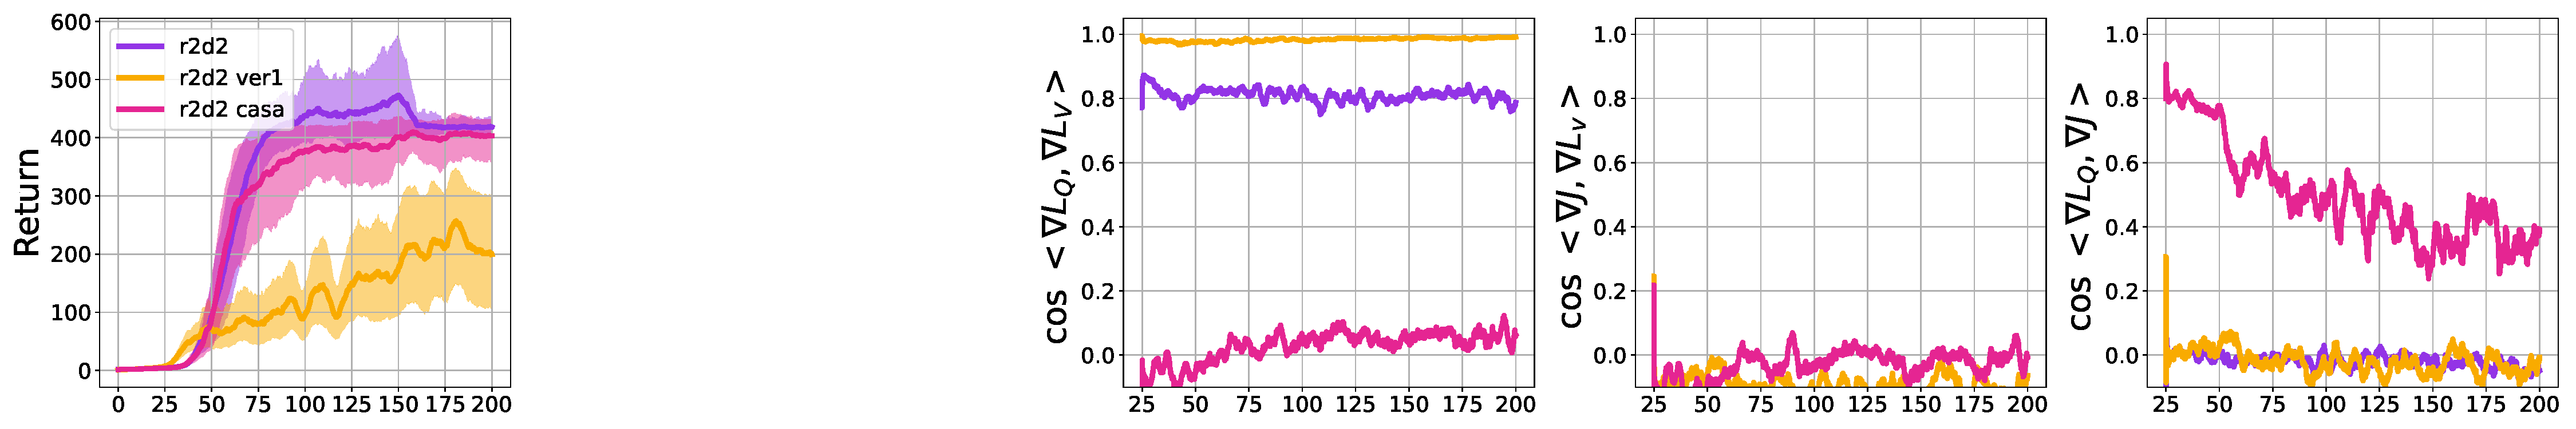
\includegraphics[width=\linewidth]{body/app_fig/app_r2d2_Breakout.pdf}


% 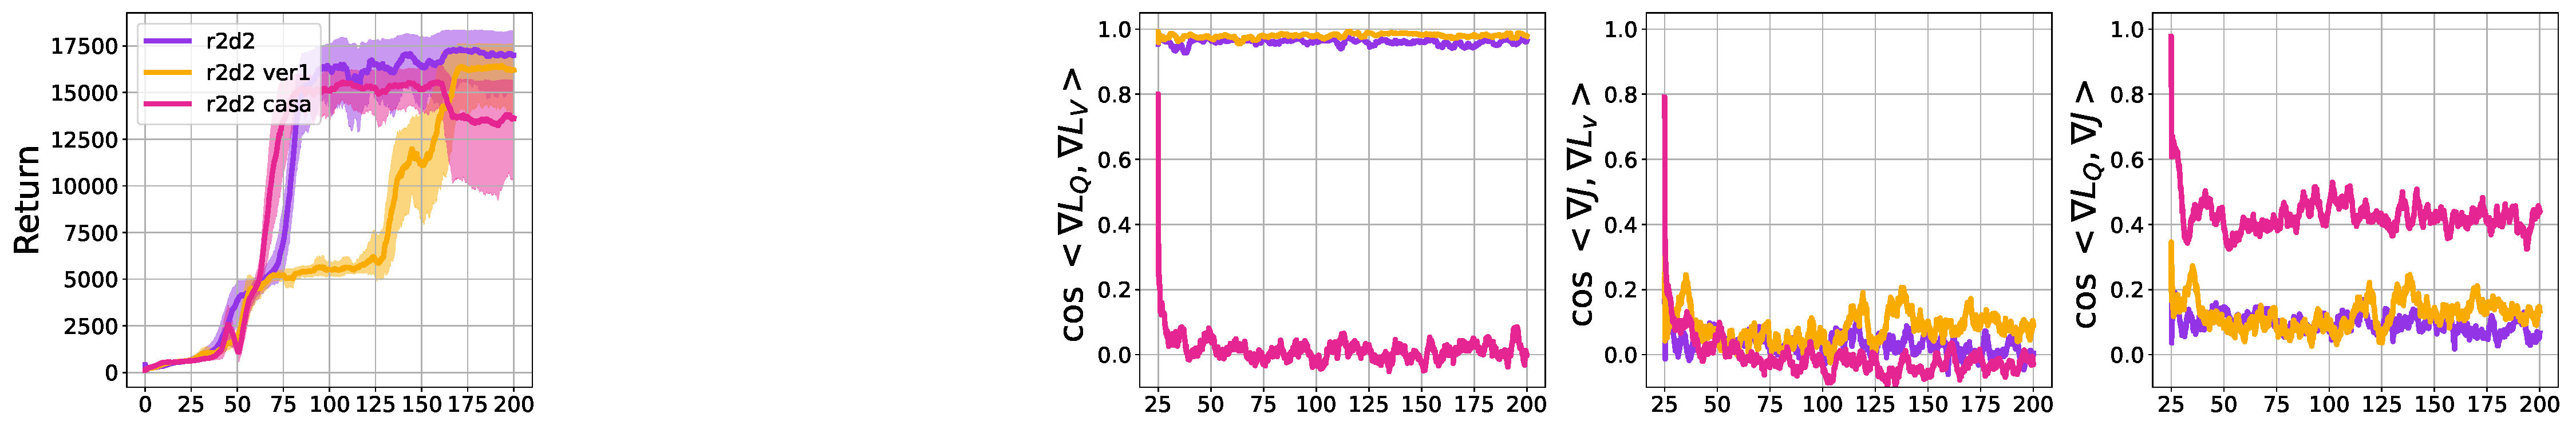
\includegraphics[width=\linewidth]{body/app_fig/app_r2d2_Qbert.pdf}
% \caption{Angles of Gradients and Returns of versions of PPO and R2D2 defined in Table \ref{tab:ppo_mtv} and Table \ref{tab:r2d2_mtv}.}
% \label{fig:mtv_app}
% \end{figure}

% \clearpage

% \changnan{casa summary deleted}
% \section{CASA summary}
% \begin{figure}[ht]
% \centering
% 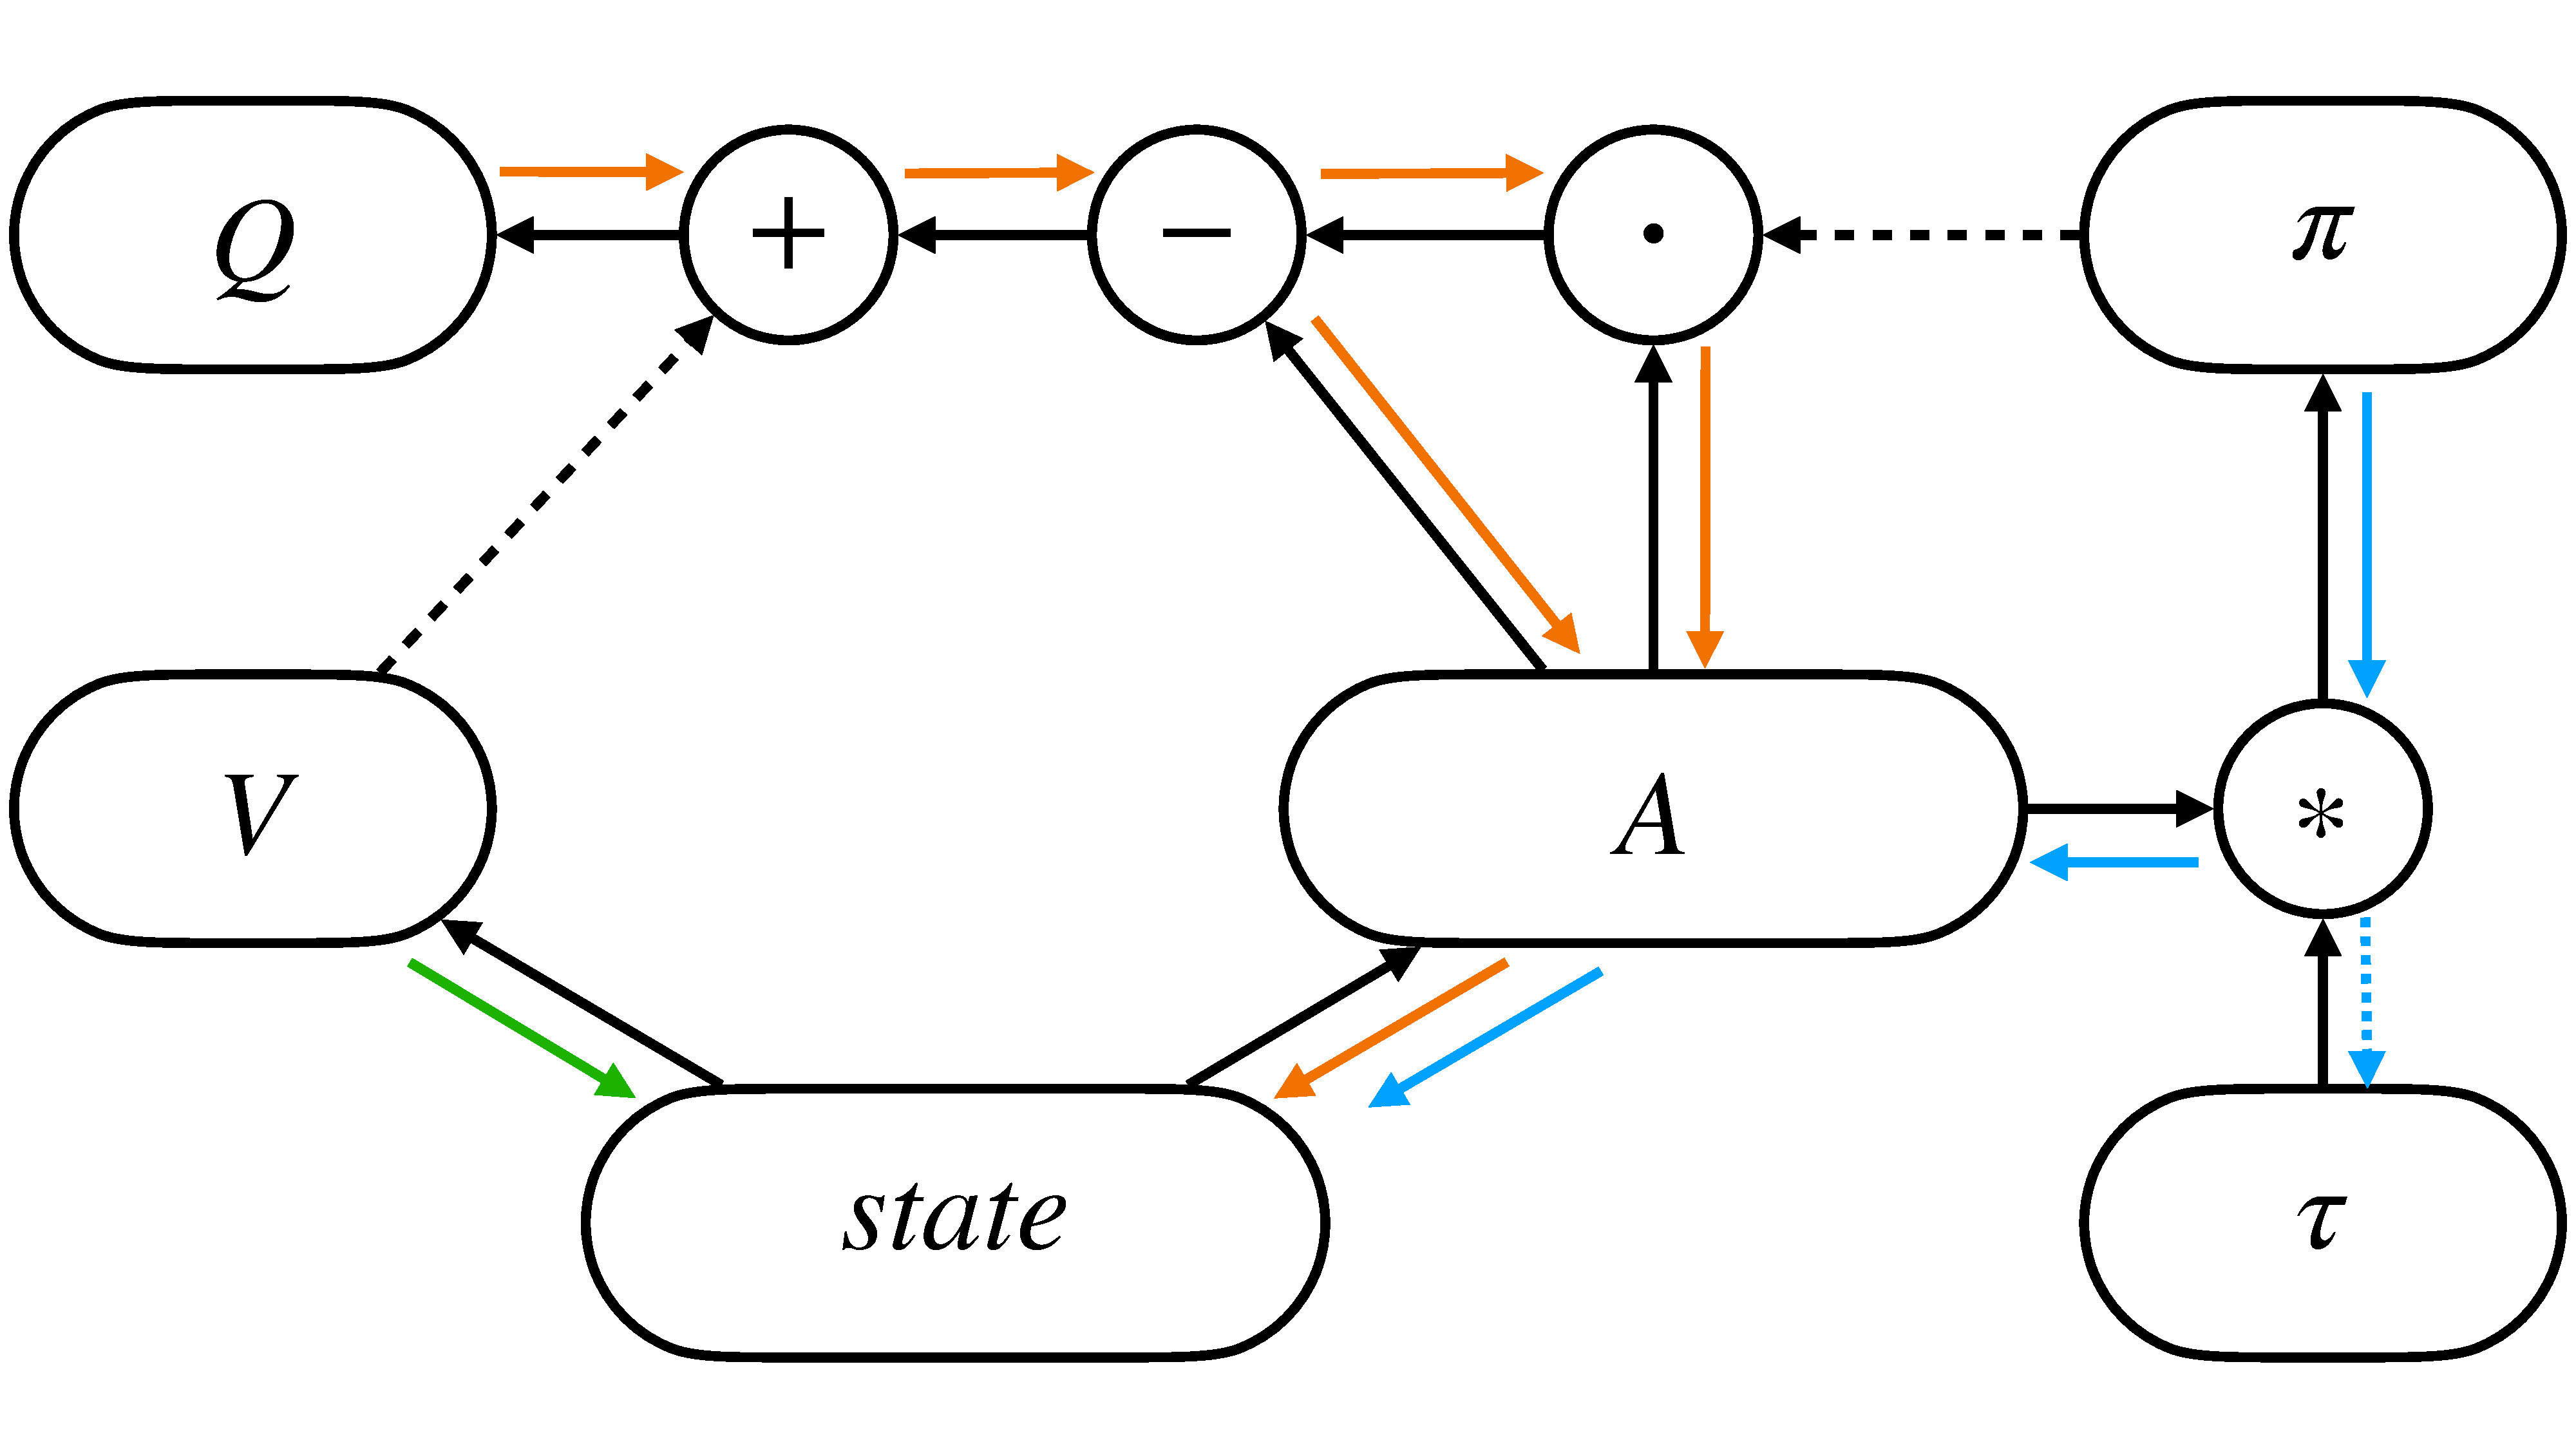
\includegraphics[width=0.4\textwidth,bb= 0 0 1800 1100]{body/figures/CASA.pdf}
% \caption{
% \textbf{Black} lines represent the forward process.
% \textbf{Dotted} black lines represent the \textit{stop gradient} operator in the forward process. 
% \textbf{Colorful} lines represent backpropagation from different loss functions. 
% Specifically, \textbf{blue} lines represent $\mathbb{E}_\pi [(Q^\pi-V)\nabla \log \pi]$, 
% \textbf{orange} lines represent $\mathbb{E}_\pi [(Q^\pi-Q)\nabla Q]$,
% and \textbf{green} lines represent $\mathbb{E}_\pi [(Q^\pi-V)\nabla V]$.}
% \label{fig:casa}
% \end{figure}
% \section{motivation experiments}

\clearpage

{\colorred \section{On Discussing Application of CASA on Continuous Action Space}
\label{app:cts_space}

As we can see CASA is only applied to discrete action space in the main context, we make a discussion on whether CASA is applicable on continuous action space. 
For brevity, we let $\tau=1$ and write \eqref{eq:casa} as:
\begin{equation}
\left\{
    \begin{aligned}
        &\pi = \text{softmax}(A), \\
        &\Bar{A} = A - \mathbb{E}_{\pi} [A], \\
        &Q = \Bar{A} + sg(V).
    \end{aligned}
\right. 
\end{equation}
The difficulty comes from estimating two quantities, one is $\text{softmax}(A)$, the other is $\mathbb{E}_{\pi} [A]$. 
This comes from the fact that discrete action space is countable so these two quantities are expressed in a closed-form, while continuous action space is uncountable so an accurate estimation of these two quantities is intractable. 
We can surely apply Monte Carlo methods to approximate, but a more elegant close-form expression may be preferred. 
Then this becomes another problem: \textit{how to estimate (state-action values / advantages / policy probabilities) of all actions in a continuous action space efficiently without loss of generality?}
This is another representational design problem, which is out of scope of this paper, so we don't touch much about it. 
But with the hope of inspiring a better solution to this problem, we provide one practical way of applying CASA on continuous action space based on kernel-based machine learning. 

Let $a_0, \dots, a_k$ to be basis actions in the action space. 
Let $A(s, a_0), \dots, A(s, a_k)$ to be advantage functions for tuples of states and basis actions. 
They can either share parameters or be isolated. 
Let $K(\cdot, \cdot)$ be a kernel function defined on the product of two action spaces. 
For any $a$ in the action space, we can estimate $A(s, a)$ by a decomposition such like $$A(s, a) = \frac{1}{Z_a} (K(a_0, a) A(s, a_0) + \dots + K(a_k, a) A(s, a_k)),$$ where $Z_a = \sum_{i=0}^k K(a_i, a)$ is a normalization constant. 

Since $K(\cdot, a)$ is a closed-form function of $a$, and $|\{A(s, a_0), \dots, A(s, a_k)\}|$ is finite, we can make a closed-form expression of both $\text{softmax}(A)$ and $\mathbb{E}_{\pi} [A]$. 
Then we can apply CASA directly on this expression, with one function estimates $V$ and the other function estimates advantages of all actions in a closed-form with only state as input.  
The policy is defined directly by $\text{softmax}$ of all advantages. 
In details, we define
\begin{equation}
\left\{
    \begin{aligned}
        &\pi(s, a) = \exp (A(s, a)) / \int_{a} \exp (A(s, a)) da, \\
        &\Bar{A}(s, a) = A(s, a) - \int_{a} sg(\pi(s, a)) A(s, a) da, \\
        &Q(s, a) = \Bar{A}(s, a) + sg(V(s)).
    \end{aligned}
\right. 
\end{equation}

Then it satisfies the consistency of CASA on continuous action space.
$$
\begin{aligned}
    \nabla \log \pi(s, a) &= \nabla A(s, a) - \frac{\nabla \int_{a} \exp (A(s, a)) da}{\int_{a} \exp (A(s, a)) da} \\
    &= \nabla A(s, a) - \frac{ \int_{a} \exp (A(s, a)) \nabla A(s, a) da}{\int_{a} \exp (A(s, a)) da} \\
    &= \nabla A(s, a) - \int_{a} \frac{  \exp (A(s, a)) }{\int_{a} \exp (A(s, a)) da} \nabla A(s, a) da \\
    &= \nabla A(s, a) - \int_{a} \pi(s, a) \nabla A(s, a) da \\
    &= \nabla \Bar{A}(s, a) = \nabla Q(s, a). 
\end{aligned}
$$
}

\section{DR-Trace}
\label{app:drtrace}

% One simple choice is to learn $V$ and $\pi$ by V-Trace \citep{impala} and to learn $Q$ by ReTrace \citep{retrace}. 
% \citep{impala} shows that $V^{\Tilde{\pi}}$ estimated by V-Trace converges to $V^*$ that corresponds to some $\Tilde{\pi}_{VTrace}$.
% Respectively, \citep{retrace} shows that $Q^{\Tilde{\pi}}$ estimated by ReTrace converges to $Q^*$ that corresponds to some $\Tilde{\pi}_{ReTrace}$.

As CASA estimates $(V, Q, \pi)$, we would ask
\textbf{i)} how to guarantee that $\Tilde{\pi}_{VTrace} = \Tilde{\pi}_{ReTrace}$, 
\textbf{ii)} how to exploit $(V, Q, \pi)$ to make a better estimation. 
Though we can apply V-Trace to estimate $V$ and ReTrace to estimate $Q$ with proper hyperparameters to guarantee $\Tilde{\pi}_{VTrace} = \Tilde{\pi}_{ReTrace}$, it's more reasonable to estimate $(V, Q)$ together. 
Inspired by Doubly Robust, which is shown to maximally reduce the variance, we introduce DR-Trace, which estimates $V$ by 
$$
\label{eq:dr-v}
    \begin{aligned}
        V_{DR}^{\Tilde{\pi}} (s_t) &\overset{def}{=} \mathbb{E}_{\mu} [ 
        V(s_t) + \sum_{k \geq 0} \gamma^k 
     c_{[t:t+k-1]} \rho_{t+k}  \delta^{DR}_{t+k} ],  
    \end{aligned}
$$
{\colorred where $\mu$ is the behavior policy}, $\delta^{DR}_t \overset{def}{=} r_t + \gamma V(s_{t+1}) - Q(s_t, a_t)$ is one-step Doubly Robust error, $\rho_t \overset{def}{=} \min\{\frac{\pi_t}{\mu_t}, \Bar{\rho} \}$ and $c_t \overset{def}{=} \min\{\frac{\pi_t}{\mu_t}, \Bar{c}\}$ are clipped per-step importance sampling, $c_{[t: t+k]} \overset{def}{=} \prod_{i=0}^{k} c_{t+i}$.

With one step Bellman equation, we estimate $Q$ by
$$
\label{eq:dr-q}
    \begin{aligned}
         Q_{DR}^{\Tilde{\pi}} (s_t, a_t) 
         &\overset{def}{=} \mathbb{E}_{s_{t+1}, r_t \sim p(\cdot, \cdot | s_t, a_t)} [  r_t + \gamma   V_{DR}^{\Tilde{\pi}} (s_{t+1}) ] 
        \\
        %  &=  \mathbb{E}_{\mu} [ r_t + \gamma V(s_{t + 1}) +
        % \gamma \sum_{k \geq 0} \gamma^k 
        % c_{[t+1:t+k]} \rho_{t+1+k}
        % \delta^{DR}_{t+1+k} V
        % ]
        % \\
        %  &= \mathbb{E}_{\mu}   [
        % Q(s_t, a_t) + \delta_t^{DR}V + \sum_{k \geq 1}  \gamma^k
        % c_{[t+1:t+k-1]} \rho_{t+k}
        % \delta^{DR}_{t+k} V
        % ],
        % \\
        &=  \mathbb{E}_{\mu}   [
        Q(s_t, a_t) + \sum_{k \geq 0}  \gamma^k
        c_{[t+1:t+k-1]} \Tilde{\rho}_{t, k}
        \delta^{DR}_{t+k}
        ], 
    \end{aligned}
$$
where $\Tilde{\rho}_{t, k} =  1_{\{k=0\}} + 1_{\{k > 0\}} \rho_{t+k}$.

% Compared to \eqref{eq:dr-v}, $c_{[t+1:t+k-1]} \Tilde{\rho}_{t, k}$ in \eqref{eq:dr-q} doesn't multiply importance sampling ratio of $a_t$, which meets the same intuition as \eqref{eq:vtrace} and \eqref{eq:retrace}.\\
\begin{theorem}
    Define $\Bar{A} = A - \mathbb{E}_\pi[A]$, $Q = \Bar{A} + sg(V)$,
    $$
    \begin{aligned}
    &\mathscr{T}(Q) \overset{def}{=} \mathbb{E}_{\mu}   [
        Q(s_t, a_t) + \sum_{k \geq 0}  \gamma^k
        c_{[t+1:t+k-1]} \Tilde{\rho}_{t, k}
        \delta^{DR}_{t+k}
        ], \\
    &\mathscr{S}(V) \overset{def}{=} \mathbb{E}_{\mu}   [
        V(s_t) + \sum_{k \geq 0}  \gamma^k
        c_{[t:t+k-1]} \rho_{t, k}
        \delta^{DR}_{t+k}
        ], \\
    &\mathscr{U}(Q, V) = (\mathscr{T}(Q) - \mathbb{E}_\pi[Q] + \mathscr{S}(V), \mathscr{S}(V)), \\
    &\mathscr{U}^{(n)}(Q, V) = \mathscr{U}(\mathscr{U}^{(n-1)}(Q, V)),
    \end{aligned}
    $$
    then $\mathscr{U}^{(n)}(Q, V) \rightarrow (Q^{\Tilde{\pi}}, V^{\Tilde{\pi}})$ that corresponds to 
    $$
        \Tilde{\pi}(a|s) = \frac
        {\min \left\{\Bar{\rho} \mu (a|s), \pi(a|s)\right\}}
        {\sum_{b \in \mathcal{A}}\min \left\{\Bar{\rho} \mu (b|s), \pi(b|s)\right\}}.
    $$ as $n \rightarrow +\infty$.
\label{thm:dr}
\end{theorem}
\begin{proof}
    See Appendix \ref{app:proof}, Theorem \ref{thm_app:dr}.
\end{proof}
Theorem \ref{thm:dr} shows that DR-Trace is a contraction mapping and $(V, Q)$ converges to $(V^{\Tilde{\pi}}, Q^{\Tilde{\pi}})$ that corresponds to 
$$
    \begin{aligned}
        \Tilde{\pi}(a|s) = \frac
        {\min \left\{\Bar{\rho} \mu (a|s), \pi(a|s)\right\}}
        {\sum_{b \in \mathcal{A}}\min \left\{\Bar{\rho} \mu (b|s), \pi(b|s)\right\}}.
    \end{aligned}
$$

% At training time, the policy evaluation is achieved by updating $\theta$ to minimize $l2$ losses
% $$
% \begin{aligned}
%     L_V(\theta) &= \mathbb{E}_\pi [ (V_\theta(s_t) -  V_{DR}^{\Tilde{\pi}} (s_t))^2 ], \\
%     L_Q(\theta) &= \mathbb{E}_\pi [ (Q_\theta(s_t, a_t) -  Q_{DR}^{\Tilde{\pi}} (s_t, a_t))^2 ],
% \end{aligned}
% $$ 
% which gives the ascent direction of $\theta$ by
% \begin{equation}
% \label{eq:grad_qv}
%     \begin{aligned}
%         \nabla_\theta L_V(\theta)
%         &= \mathbb{E}_\pi \left[ (V_{DR}^{\Tilde{\pi}} (s_t) - V_\theta(s_t) ) \nabla V_\theta(s_t) \right], \\
%         \nabla_\theta L_Q(\theta)
%         &= \mathbb{E}_\pi \left[ (Q_{DR}^{\Tilde{\pi}} (s_t, a_t) - Q_\theta(s_t, a_t)) \nabla Q_\theta(s_t, a_t) \right].
%     \end{aligned}
% \end{equation}
% And we make the policy improvement by policy gradient, which gives the ascent direction of $\theta$ by 
% \begin{equation}
% \label{eq:grad_pi}
% \begin{aligned}
%     \nabla_\theta \mathcal{J}(\tau, \theta) = \mathbb{E}_\mu \left[\tau \rho_t (Q_{DR}^{\Tilde{\pi}} (s_t, a_t) - V_\theta(s_t) ) \nabla_\theta \log \pi_t \right],
% \end{aligned}
% \end{equation}
% where $\mathcal{J} (\tau, \theta) = \tau \mathbb{E}_\pi [\sum \gamma^t r_t]$.
% It takes an additional $\tau$, which frees the scale of gradient from $\tau$.

% Finally, the gradient ascent direction of $\theta$ is given by
% \begin{equation}
%     \label{eq:grad_all}
%     \alpha_1 \nabla_\theta L_V + \alpha_2 \nabla_\theta L_Q + \alpha_3 \nabla_\theta \mathcal{J}.
% \end{equation}

% \textbf{Full algorithm is described in Appendix \ref{app:casa}.}
% Note that \eqref{eq:grad_all} doesn't need any entropy regularization. 
% We will discuss why this happens in section \ref{sec:equiv} and how CASA controls the exploration in section \ref{sec:ent_control}.


\begin{figure}[h]
    \centering
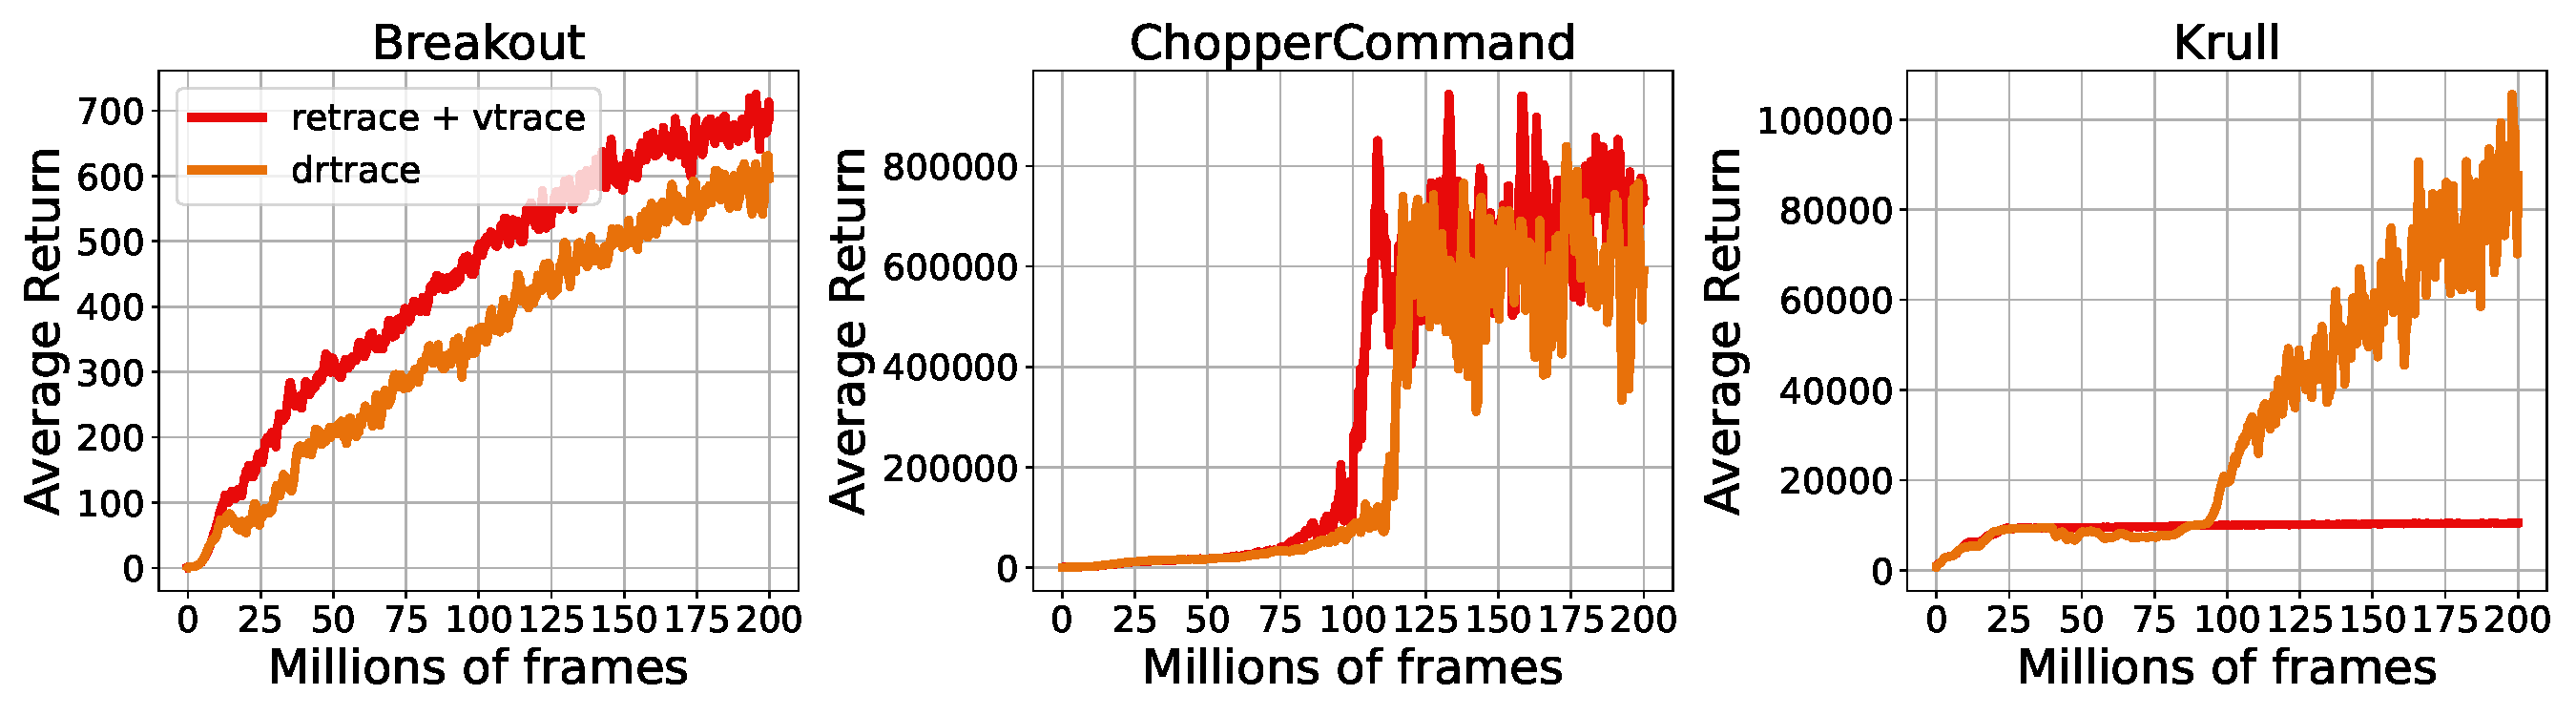
\includegraphics[width=\linewidth]{body/ablation/dr_ablation.pdf}
    \caption{Ablation study for w/wo DR-Trace on Breakout, ChopperCommand and Krull.}
    \label{fig:app_dr_trace}
\end{figure}

According to our proof, DR-Trace should work similar to V-Trace and ReTrace, as the convergence rate and the limitation are same. 
We compare DR-Trace with V-Trace+ReTrace in Figure \ref{fig:app_dr_trace}, where we replace estimation of state values by V-Trace and estimation of state-action values by ReTrace. 
We call V-Trace+ReTrace as No-DR-Trace for brevity. 
No-DR-Trace performs better on Breakout and ChopperCommand, but fails to make a breakthrough on Krull. 
Recalling the fact that Doubly Robust can maximally reduce the variance of Bellman error, No-DR-Trace is less stable but also potential to achieve a better performance. 
A conclusion cannot be made about No-DR-Trace, as this phenomenon means that No-DR-Trace is less stable than DR-Trace, but it also holds the potential to achieve a better performance.

% \clearpage


\section{Proofs}
\label{app:proof}

\theoremstyle{plain}
% \setcounter{Lemma}{0}
\newtheorem{Lemma_app}{Lemma}[section]
\newtheorem{Theorem_app}{Theorem}[section]
\theoremstyle{definition}
\newtheorem*{Remark_app}{Remark}
\theoremstyle{remark}

% \begin{Lemma_app}
% Let 
% $g \in \textbf{C}^{1}(\mathbb{R}^{n}): \mathbb{R}^{n} \to \mathbb{R}^{n}, \ f \in \textbf{C}^{1}(\mathbb{R}^{n+k}): \mathbb{R}^{n+k} \to \mathbb{R}^{n}.
% $\\
% If
% $
% \nabla_x g(x) = \nabla_x f(x, y)$, for $\forall x\in \mathbb{R}^{n}, y\in \mathbb{R}^k,
% $
% then $\exists$ $c \in \textbf{C}^{1}(\mathbb{R}^{k}): \mathbb{R}^{k} \to \mathbb{R}^{n}$, s.t. $f(x, y) = g(x) + c(y)$.
% \label{lemma_app:func_sep}
% \end{Lemma_app}
% \begin{proof}

% Let $\Tilde{f}(x, y) = f(x, y) - g(x)$.

% Since $\nabla_x g(x) = \nabla_x f(x, y)$, we have 
% $$
% \nabla_x \Tilde{f} = 0, \ for \ \forall x\in \mathbb{R}^{n}, y\in \mathbb{R}^k.
% $$

% So $\Tilde{f}$ is a constant function w.r.t $x$, which can be denoted as $c(y) = \Tilde{f}(x, y)$.

% Hence, $f(x, y) = g(x) + c(y)$.
% \end{proof}

\begin{Lemma_app}
(i) Define $\pi = softmax(A / \tau)$, then $\nabla \log \pi = (\textbf{1} - \pi) \frac{\nabla A}{\tau}$. 
(ii) Denote $sg$ to be stop gradient and define $\Bar{A} = A - \mathbb{E}_\pi [A]$, $Q = \Bar{A} + sg(V)$, then $\nabla Q = (\textbf{1} - \pi) \nabla A$.
\label{lemma_app:vannila_grad}
\end{Lemma_app}
\begin{proof}

As $Q = \Bar{A} + sg(V) = A - sg(\pi)\cdot A + sg(V)$, it's obvious that $\nabla Q = (\textbf{1} - \pi) \nabla A$.

For $\log \pi$, it's a standard derivative of cross entropy, so we have $\nabla \log \pi = (\textbf{1} - \pi) \nabla (A / \tau) = (\textbf{1} - \pi) \frac{\nabla A}{\tau}$.
\end{proof}

\begin{Lemma_app}
Define $\Bar{A}= A - \mathbb{E}_\pi[A]$, $Q = \Bar{A} + sg(V), \pi = softmax(A / \tau)$, then 
$$
\mathbb{E}_\pi \left[ (Q - V) \nabla \log \pi \right]
= - \tau \nabla \textbf{H}[\pi].
$$
\label{lemma_app:eqiv_pg_ent}
\end{Lemma_app}
\begin{proof}
Since 
$$
\pi = \exp(A / \tau) / Z,\ Z = \int_\mathcal{A} \exp(A / \tau),
$$
we have 
$$
A = \tau \log \pi + \tau \log Z.
$$
Based on the observation that $\mathbb{E}_\pi \left[ f(s) \nabla \log \pi (\cdot | s) \right] = 0$, 
we have 
$$\mathbb{E}_\pi \left[ \mathbb{E}_\pi[A] \cdot \nabla \log \pi \right] = 0,$$ 
$$\mathbb{E}_\pi \left[ \log Z \cdot \nabla \log \pi \right] = 0.$$

On the one hand,
$$
\begin{aligned}
    \mathbb{E}_\pi \left[ (Q - V) \nabla \log \pi \right]
    &= \mathbb{E}_\pi \left[ A \nabla \log \pi \right] 
    - \mathbb{E}_\pi \left[ \mathbb{E}_\pi[A] \cdot \nabla \log \pi \right] \\
    &= \tau \mathbb{E}_\pi \left[ \log \pi \nabla \log \pi \right]
    + \tau \mathbb{E}_\pi \left[ \log Z \cdot \nabla \log \pi \right] \\
    &= \tau \mathbb{E}_\pi \left[ \log \pi \nabla \log \pi \right].
\end{aligned}
$$

On the other hand, 
$$
\begin{aligned}
    \nabla \textbf{H} [\pi] 
    &= - \nabla \int_\mathcal{A} \pi_i \log \pi_i \\
    &= - \int_\mathcal{A}  \nabla \pi_i \cdot \log \pi_i - \int_\mathcal{A} \pi_i \nabla \log \pi_i  \\
    &= - \int_\mathcal{A}  \pi_i \nabla \log \pi_i \cdot \log \pi_i - \int_\mathcal{A}  \pi_i \frac{\nabla \pi_i}{\pi_i} \\
    &= - \mathbb{E}_\pi \left[ \log \pi \nabla \log \pi \right].
\end{aligned}
$$
Hence, $
\mathbb{E}_\pi \left[ (Q - V) \nabla \log \pi \right]
= - \tau \nabla \textbf{H}[\pi]
$.
\end{proof}

\begin{Theorem_app}
    Define $\Bar{A} = A - \mathbb{E}_\pi[A]$, $Q = \Bar{A} + sg(V)$.
    Define $$
    \begin{aligned}
    &\mathscr{T}(Q) \overset{def}{=} \mathbb{E}_{\mu}   [
        Q(s_t, a_t) + \sum_{k \geq 0}  \gamma^k
        c_{[t+1:t+k-1]} \Tilde{\rho}_{t, k}
        \delta^{DR}_{t+k}
        ], \\
    &\mathscr{S}(V) \overset{def}{=} \mathbb{E}_{\mu}   [
        V(s_t) + \sum_{k \geq 0}  \gamma^k
        c_{[t:t+k-1]} \rho_{t, k}
        \delta^{DR}_{t+k}
        ], \\
    &\mathscr{U}(Q, V) = (\mathscr{T}(Q) - \mathbb{E}_\pi[Q] + \mathscr{S}(V), \mathscr{S}(V)), \\
    &\mathscr{U}^{(n)}(Q, V) = \mathscr{U}(\mathscr{U}^{(n-1)}(Q, V)),
    \end{aligned}
    $$
    then $\mathscr{U}^{(n)}(Q, V) \rightarrow (Q^{\Tilde{\pi}}, V^{\Tilde{\pi}})$ that corresponds to 
    $$
        \Tilde{\pi}(a|s) = \frac
        {\min \left\{\Bar{\rho} \mu (a|s), \pi(a|s)\right\}}
        {\sum_{b \in \mathcal{A}}\min \left\{\Bar{\rho} \mu (b|s), \pi(b|s)\right\}}.
    $$ as $n \rightarrow +\infty$.
\label{thm_app:dr}
\end{Theorem_app}
\begin{Remark_app}
$\mathscr{T}(Q) - \mathbb{E}_\pi[Q] + \mathscr{S}(V)$ is \textbf{exactly} how $Q$ is updated at training time. 
Since $Q = \Bar{A} + sg(V)$, if we apply gradient ascent on $Q$ and $V$ in directions $\nabla L_Q(\theta)$ and $\nabla L_V(\theta)$ respectively, change of $Q$ comes from two aspects. One comes from $\nabla L_Q(\theta)$, which changes $A$, the other comes from $\nabla L_V(\theta)$, which changes $V$. Because the gradient of $V$ is stopped when estimating $Q$, the latter is captured by "minus old baseline, add new baseline", which is $- \mathbb{E}_\pi[Q] + \mathscr{S}(V)$ in Theorem \ref{thm_app:dr}.
\end{Remark_app}
\begin{proof}
 Define
 $$
 \begin{aligned}
        \widetilde{\mathscr{T}}(Q) &= - \mathbb{E}_\pi[Q] + \mathscr{T}(Q), \\
        \widetilde{\mathscr{U}}(Q, V) &= (\widetilde{\mathscr{T}}(Q), \mathscr{S}(V)), \\
        \widetilde{\mathscr{U}}^{(n)}(Q, V) &=   \widetilde{\mathscr{U}}(\widetilde{\mathscr{U}}^{(n-1)}(Q, V)).
 \end{aligned}
 $$
By Lemma \ref{lemma_app:dr_q}, $\widetilde{\mathscr{T}}^{(n)}(Q)$ converges to some $A^*$ as $n \rightarrow \infty$. This process will not influence the estimation of $V$ as the gradient of $V$ is stopped when estimating $Q$. According to the proof, $A^*$ does not depend on $V$. \\
By Lemma \ref{lemma_app:dr_v}, $\mathscr{S}^{(n)}(V)$ converges to some $V^*$ as $n \rightarrow \infty$. \\
Hence, we have
$$
\widetilde{\mathscr{U}}^{(n)}(Q, V) \rightarrow (A^*, V^*)\ \ as\ \ n \rightarrow +\infty. 
$$
By definition, 
$$
\mathscr{U}(Q, V) = (\widetilde{\mathscr{T}}(Q) + \mathscr{S}(V), \mathscr{S}(V)),
$$
we can regard $\widetilde{\mathscr{T}}(Q) + \mathscr{S}(V)$ as $Q$ and regard $\mathscr{S}(V)$ as $V$, then
$$
\begin{aligned}
    \mathscr{U}^{(2)}(Q, V) 
    &= \mathscr{U}(\widetilde{\mathscr{T}}(Q) + \mathscr{S}(V), \mathscr{S}(V)) \\
    &= (\mathscr{T}(\widetilde{\mathscr{T}}(Q) + \mathscr{S}(V)) -\mathscr{S}(V) + \mathscr{S}^{(2)}(V), \mathscr{S}^{(2)}(V)) \\
    &= (\widetilde{\mathscr{T}}^{(2)}(Q) + \mathscr{S}^{(2)}(V), \mathscr{S}^{(2)}(V)).
\end{aligned}
$$
By induction, 
$$
\begin{aligned}
    \mathscr{U}^{(n)}(Q, V) &= (\widetilde{\mathscr{T}}^{(n)}(Q) + \mathscr{S}^{(n)}(V), \mathscr{S}^{(n)}(V)) \\
    &\rightarrow (A^*+V^*, V^*)\ \ as\ \ n\rightarrow + \infty.
\end{aligned}
$$
Same as \citep{impala}, 
$$
    \Tilde{\pi}(a|s) = \frac
    {\min \left\{\Bar{\rho} \mu (a|s), \pi(a|s)\right\}}
    {\sum_{b \in \mathcal{A}}\min \left\{\Bar{\rho} \mu (b|s), \pi(b|s)\right\}}.
$$ 
is the policy s.t. the Bellman equation holds, which is 
$$\mathbb{E}_\mu[\rho_t (r_t + \gamma V_{t+1} - V_t) | \mathscr{F}_t] = 0,$$ and $\mathscr{U}(Q^{\Tilde{\pi}}, V^{\Tilde{\pi}}) = (Q^{\Tilde{\pi}}, V^{\Tilde{\pi}})$. \\
So we have
$(A^*+V^*, V^*) = (Q^{\Tilde{\pi}}, V^{\Tilde{\pi}}).$
\end{proof}

\begin{Lemma_app}
Define $\Bar{A}= A - \mathbb{E}_\pi[A]$, $Q = \Bar{A} + sg(V)$,
then operator 
$$
    \mathscr{T}(Q) \overset{def}{=} \mathbb{E}_{\mu}   [
        Q(s_t, a_t) + \sum_{k \geq 0}  \gamma^k
        c_{[t+1:t+k-1]} \Tilde{\rho}_{t, k}
        \delta^{DR}_{t+k}
        ]
$$
is a contraction mapping w.r.t. $Q$.
\label{lemma_app:dr_q}
\end{Lemma_app}
\begin{Remark_app}
Note that $\mathscr{T}(Q)$ is exactly \eqref{eq:dr-q}. 

Since $Q = A + sg(V)$, the gradient of $V$ is stopped when estimating $Q$, updating $Q$ will not change $V$, which is equivalent to updating $A$.
Without loss of generality, we assume $V$ is fixed as $V^*$ in the proof.
\end{Remark_app}
\begin{proof}

$\Bar{A} = A - \mathbb{E}_\pi[A]$ shows $\mathbb{E}_\pi[\Bar{A}] = 0$, which guarantees that no matter how we update $A$, we always have $\mathbb{E}_\pi[Q] = V^*$.

Based on above observations, define 
$$
    \widetilde{\mathscr{T}}(Q) \overset{def}{=} - \mathbb{E}_\pi [Q] + \mathscr{T}(Q).
$$

It's obvious that we only need to prove $\widetilde{\mathscr{T}}(Q)$ is a contraction mapping.

For brevity, we denote $$Q_t = Q(s_t, a_t), A_t = A(s_t, a_t), V^*_t = V^*(s_t).$$

Noticing that $\Tilde{\rho}_{t, 0} = 1$, let $\mathscr{F}$ represent filtration, we can rewrite $\widetilde{\mathscr{T}}$ as 
\begin{equation}
\label{eq:dr_a_2}
\begin{aligned}
    \widetilde{\mathscr{T}}(Q)
    &= \mathbb{E}_{\mu}   [
        A_t + \sum_{k \geq 0}  \gamma^k
        c_{[t+1:t+k-1]} \Tilde{\rho}_{t, k}
        \delta^{DR}_{t+k}
        ] \\
    &= \mathbb{E}_{\mu}   [
        -V^*_t + \sum_{k \geq 0}  \gamma^k
        c_{[t+1:t+k-1]} \Tilde{\rho}_{t, k}
        r_{t+k}
        + 
        \sum_{k \geq 0}  \gamma^{k+1}
        c_{[t+1:t+k-1]} \Delta_k ],
        \\
\end{aligned}
\end{equation}
where 
\begin{equation}
\label{eq:dr_delta}
    \Delta_k = \mathbb{E}_{\mu}\left[\Tilde{\rho}_{t, k} V^*_{t+k+1} - c_{t+k} \Tilde{\rho}_{t, k+1} Q_{t+k+1} | \mathscr{F}_{t+k}\right].
\end{equation}
By definition of $Q$,
$$
    \mathbb{E}_{\mu}[V_{t+k+1}^*|\mathscr{F}_{t+k}] 
    = \mathbb{E}_{\mu}[
    \mathbb{E}_\pi[Q_{t+k+1}|\mathscr{F}_{t+k+1}]
    |\mathscr{F}_{t+k}], \\
    % \geq&  \mathbb{E}_{\mu}[
    % \mathbb{E}_\mu[\Tilde{\rho}_{t, k+1} Q_{t+k+1}|\mathscr{F}_{t+k+1}]
    % |\mathscr{F}_{t+k}], 
$$
we can rewrite \eqref{eq:dr_delta} as
\begin{equation}
\label{eq:dr_q_delta}
\Delta_k = \mathbb{E}_{\mu}[
(
\Tilde{\rho}_{t, k} \frac{\pi_{t+k+1}}{\mu_{t+k+1}}- c_{t+k} \Tilde{\rho}_{t, k+1} 
) Q_{t+k+1} | \mathscr{F}_{t+k}
].
\end{equation}
For any $Q_1 = A_1 + sg(V^*)$, $Q_2 = A_2 + sg(V^*)$, since
$$
\mathbb{E}_{\mu}[
(
\Tilde{\rho}_{t, k} \frac{\pi_{t+k+1}}{\mu_{t+k+1}}- c_{t+k} \Tilde{\rho}_{t, k+1} 
) | \mathscr{F}_{t+k}
] \geq 0,
$$
by \eqref{eq:dr_a_2} \eqref{eq:dr_q_delta}, we have 
% $$
% || \Delta^1_k - \Delta_k^2 || \leq \mathbb{E}_{\mu}\left[
% \left(
% \Tilde{\rho}_{t, k} \frac{\pi_{t+k+1}}{\mu_{t+k+1}}- c_{t+k} \Tilde{\rho}_{t, k+1} 
% \right) | \mathscr{F}_{t+k}
% \right] ||A^1 - A_2||.
% $$
$$
        || \widetilde{\mathscr{T}}(Q_1) - \widetilde{\mathscr{T}}(Q_2) || 
        % \leq& \mathbb{E}_{\mu} \left[ \sum_{k \geq 0}  \gamma^{k+1} c_{[t+1:t+k-1]} || \Delta_k^1 - \Delta_k^2 || \right] \\
        \leq \mathcal{C} || Q_1 - Q_2 ||,
$$
where 
$$
    \begin{aligned}
        \mathcal{C} 
        &= \mathbb{E}_{\mu} [ \sum_{k \geq 0}  \gamma^{k+1} c_{[t+1:t+k-1]} 
        (
        \Tilde{\rho}_{t, k} \frac{\pi_{t+k+1}}{\mu_{t+k+1}}- c_{t+k} \Tilde{\rho}_{t, k+1} 
        ) ]
        \\
        &= \mathbb{E}_{\mu} [1 -1 + \sum_{k \geq 0}  \gamma^{k+1} c_{[t+1:t+k-1]} 
        \left(
        \Tilde{\rho}_{t, k} - c_{t+k} \Tilde{\rho}_{t, k+1} 
        \right) ] 
        \\
        &= 1 - (1 - \gamma)  \mathbb{E}_{\mu} [\sum_{k \geq 0} \gamma^{k}c_{[t+1:t+k-1]} \Tilde{\rho}_{t, k}  ] \\
        &\leq 1 - (1 - \gamma) < 1.
    \end{aligned}
$$
Hence, $\widetilde{\mathscr{T}}(Q)$ is a contraction mapping and converges to some fixed function, which we denote as $A^*$. So $\mathscr{T}(Q)$ is also a contraction mapping and converges to $A^*+V^*$.
\end{proof}

\begin{Lemma_app}
Define $Q = A + sg(V)$ with $\mathbb{E}_\pi [A] = 0$,
then operator 
$$
    \mathscr{S}(V) \overset{def}{=} \mathbb{E}_{\mu}  [
        V(s_t) + \sum_{k \geq 0}  \gamma^k
        c_{[t:t+k-1]} \rho_{t, k}
        \delta^{DR}_{t+k}
        ]
$$
is a contraction mapping w.r.t. $V$.
\label{lemma_app:dr_v}
\end{Lemma_app}
\begin{Remark_app}
Note that $\mathscr{S}(V)$ is exactly \eqref{eq:dr-v}. 
\end{Remark_app}
\begin{proof}

% Since $Q = A + sg(V)$, updating $V$ wouldn't influence $A$. WLOG, we assume $A$ is fixed as $A^*$ in Lemma \ref{lemma_app:dr_v}. \\
Same as Lemma \ref{lemma_app:dr_q}, we can get
$$
    \Delta_k = \mathbb{E}_{\mu}\left[
    \left( \rho_{t+k} - c_{t+k} \rho_{t+k+1}\right) V_{t+k+1} 
     -  c_{t+k} \rho_{t+k+1} A^*_{t+k+1} | \mathscr{F}_{t+k}\right],
$$
so we have 
$$
    \Delta^1_k - \Delta^2_k = \mathbb{E}_{\mu}\left[ 
    \left( \rho_{t+k} - c_{t+k} \rho_{t+k+1}\right) \cdot  
   (V^1_{t+k+1} -  V^2_{t+k+1})
     | \mathscr{F}_{t+k}\right].
$$
The remaining proof is identical to \citep{impala}'s.
\end{proof}

% \clearpage

% \begin{Lemma_app}
% Let $v \in \mathbb{R}^{|\mathcal{A}|}$ to be a vector. 
% Define 
% $
%     \pi (\tau) = \exp (v / \tau) / Z,\  Z = \int_\mathcal{A}  \exp(v / \tau).
% $
% Let $\Omega$ to be a probability measure supported on $[K, +\infty]$,
% then $f(\Omega) = \mathbb{E}_{\tau \sim \Omega} [\mathbb{E}_{\pi(\tau)} [v]]$ satisfies Lipschitz-1 condition with Wasserstein-1 metric.
% \label{lemma_app:lips}
% \end{Lemma_app}
% \begin{proof}
% Without loss of generality, we assume $v_1 \geq v_2 \geq ... \geq v_{|\mathcal{A}|}$.

% For any $\tau \in [0, +\infty)$, since
% $$
% \begin{aligned}
%     \pi (\tau) = \exp (v / \tau) / Z,\  Z = \int_\mathcal{A}  \exp(v / \tau),
% \end{aligned}
% $$
% we have
% $$
%     v = \tau \log \pi (\tau) + \tau \log Z.
% $$

% Denote $\Tilde{v}_j = v_j / \tau$. \\
% Since 
% $$
% \frac{\partial \log \pi_i}{\partial \Tilde{v}_j} = 1_{i=j} - \pi_j,
% $$
% we have
% $$
% \begin{aligned}
%     \frac{\partial \log \pi_i}{\partial \tau} 
%     &= \sum_j \frac{\partial \log \pi_i}{\partial \Tilde{v}_j} \cdot \frac{\partial \Tilde{v}_j}{\partial \tau} \\
%     &= - \sum_j (1_{i=j} - \pi_j) \frac{v_j}{\tau^2} \\
%     &= - \frac{1}{\tau^2} ( v_i - \sum_j \pi_j v_j ) \\ 
%     &= - \frac{1}{\tau^2} \left( v_i - \mathbb{E}_\pi [v] \right). 
% \end{aligned}
% $$
% Therefore, we have
% $$
% \begin{aligned}
%     \frac{\partial \pi_i}{\partial \tau} 
%     &= \pi_i \frac{\partial \log \pi_i}{\partial \tau} \\
%     &= - \frac{\pi_i}{\tau^2} \left( v_i - \mathbb{E}_\pi [v] \right).
% \end{aligned}
% $$
% Let $f(\tau) = v \cdot \pi(\tau)$, then
% $$
% \frac{\partial f}{\partial \tau} = - \frac{1}{\tau^2} \sum_i v_i \pi_i \left( v_i - \mathbb{E}_\pi [v] \right).
% $$
% Since $\sum_i \mathbb{E}_\pi [v] \pi_i \left( v_i - \mathbb{E}_\pi [v] \right) = 0$,
% we know
% $$
% \begin{aligned}
%     \frac{\partial f}{\partial \tau} 
%     &= - \frac{1}{\tau^2} \sum_i \left( v_i - \mathbb{E}_\pi [v] \right) \pi_i \left( v_i - \mathbb{E}_\pi [v] \right) \\
%     &= - \frac{1}{\tau^2} \sum_i \pi_i \left( v_i - \mathbb{E}_\pi [v] \right)^2 \\
%     &= - \frac{1}{\tau^2} \textbf{Var}_\pi [v].
% \end{aligned}
% $$
% It's obvious that
% $$
% \left| \frac{\partial f}{\partial \tau} \right| \leq \frac{1}{K^2} |v_1 - v_{|\mathcal{A}|}|^2.
% $$
% Hence, for any $\tau_1, \tau_2 \in [K, +\infty]$,
% $$
% |v \cdot \pi(\tau_1) - v \cdot \pi(\tau_2)| \leq C | \tau_1 - \tau_2|.
% $$

% Finally, for any $\gamma \in \Gamma(\Omega_1, \Omega_2)$ \footnote{$\Gamma(\Omega_1, \Omega_2)$ is the collection of all measures on $[K, +\infty] \times [K, +\infty]$ with marginals $(\Omega_1, \Omega_2)$.}, we have
% $$
% \begin{aligned}
% \left| \mathbb{E}_{\tau_1 \sim \Omega_1} [v \cdot \pi (\tau_1)] - \mathbb{E}_{\tau_2 \sim \Omega_2} [v \cdot \pi (\tau_2)] \right|
% &= \left| \int_{[K, +\infty] \times [K, +\infty]} (v \cdot \pi (\tau_1) - v \cdot \pi (\tau_2)) d \gamma (\tau_1, \tau_2) \right| \\
% &\leq \int_{[K, +\infty] \times [K, +\infty]} |v \cdot \pi (\tau_1) - v \cdot \pi (\tau_2)| d \gamma (\tau_1, \tau_2) \\
% &\leq C \int_{[K, +\infty] \times [K, +\infty]} |\tau_1 - \tau_2| d \gamma (\tau_1, \tau_2).
% \end{aligned}
% $$

% Taking infimum over $\Gamma(\Omega_1, \Omega_2)$, we have
% $$
% \left| \mathbb{E}_{\tau_1 \sim \Omega_1} [v \cdot \pi (\tau_1)] - \mathbb{E}_{\tau_2 \sim \Omega_2} [v \cdot \pi (\tau_2)] \right|
% \leq C W_1 (\Omega_1, \Omega_2),
% $$

% which proves that $f(\Omega) = \mathbb{E}_{\tau \sim \Omega} [\mathbb{E}_{\pi (\tau)} [v]]$ satisfies Lipschitz-1 condition with Wasserstein-1 metric.

% \end{proof}

\clearpage

\section{Hyperparameters}
\label{app:hyperparameters}

Our python packages are shown in Table \ref{tab:package}.


\begin{table}[h!]
\begin{center}
\begin{tabular}{l@{\hspace{.43cm}}l@{\hspace{.22cm}}}
\toprule
\textbf{Package} & \textbf{Version}  \\
\midrule
ale-py & 0.6.0.dev20200207 \\
gym & 0.19.0 \\
tensorflow & 1.15.2 \\
opencv-python & 4.1.2.30 \\
opencv-contrib-python & 4.4.0.46 \\
\bottomrule
\end{tabular}
\caption{Versions for python packages among all experiments.}
\label{tab:package}
\end{center}
\end{table}

All experiments follow the shared hyperparameters as in Table \ref{tab:shared_hyperparameters}. 
The specific hyperparameters for PPO, R2D2 and CASA+DR-Trace are shown in Table \ref{tab:ppo_hyperparameters}, Table \ref{tab:r2d2_hyperparameters} and Table \ref{tab:drtrace_hyperparameters}.
The only exceptions are $V$-loss scaling, $Q$-loss scaling and $\pi$-loss scaling, which may be zero depending on some specific ablation settings. 
We will state these three hyperparameters every time in all experiments.

% \begin{multicols}{2}
\begin{table}[H]
\begin{center}
\scalebox{0.95}{
\begin{tabular}{l@{\hspace{.43cm}}l@{\hspace{.22cm}}}
\toprule
\textbf{Parameter} & \textbf{Value}  \\
\midrule
Atari Version & NoFrameskip-v4 \\
Atari Wrapper & gym.wrappers.atari\_preprocessing \\
Image Size & (84, 84) \\
Grayscale & Yes \\
Num. Action Repeats & 4 \\
Num. Frame Stacks & 4 \\
Action Space & Full \\
End of Episode When Life Lost & No \\
% Num. States & 200M \\
Num. Environments & 160 \\
% Reward Clip & Yes \\
% Intrinsic Reward & No \\
Random No-ops & 30 \\
% Burn-in & 40 \\
% Seq-length & 80 \\
Burn-in Stored Recurrent State & Yes \\
Bootstrap & Yes \\
Optimizer & Adam Weight Decay \\
Weight Decay Rate & 0.01 \\
Weight Decay Schedule & Anneal linearly to 0 \\
Learning Rate & 5e-4 \\
Warmup Steps & 4000 \\
Learning Rate Schedule & Anneal linearly to 0 \\
AdamW $\beta_1$ & 0.9 \\
AdamW $\beta_2$ & 0.98 \\
AdamW $\epsilon$ & 1e-6 \\
AdamW Clip Norm & 50.0 \\
% Auxiliary Forward Dynamic Task & Yes \\
% Auxiliary Inverse Dynamic Task & Yes \\
Learner Push Model Every $n$ Steps & 25 \\
Actor Pull Model Every $n$ Steps & 64 \\
% Num. Bandits & 7 \\
% Bandit Learning Rate & Uniform([0.05, 0.1, 0.2]) \\
% Bandit Tiling Width & Uniform([1, 2, 3]) \\
% Num. Bandit Candidates & 7 \\
% Bandit Value Normalization & Yes \\
% Bandit UCB Scaling & 1.0 \\
% Bandit Search Range for $1 / \tau$ & [0.0, 50.0] \\
\bottomrule
\end{tabular}}
\caption{Configurations for shared hyperparameters among all experiments.}
\label{tab:shared_hyperparameters}
\end{center}
\end{table}
% \end{multicols}

% \section{Preprocess setting}
% \label{app:preprocess}
% \haosen{should we add some gym version and other details for reproducibility?}

\clearpage



% \begin{table}[H]
% \begin{center}
% \caption{Shared Hyperparameters for All Experiments.}
% \label{tab:fixed_model_hyper-parameters_atari}
% \resizebox{\textwidth}{!}{% <------ Don't forget this %
%  \begin{tabular}{l l l l }
% \toprule
% \textbf{Parameter} & \textbf{Value} & \textbf{Parameter} & \textbf{Value}  \\
% \midrule
% Image Size & (84, 84) & Grayscale & Yes \\
% Num. Action Repeats & 4 &  Num. Frame Stacks & 4 \\
% Action Space & Full & End of Episode When Life Lost & No \\
% Num. States & 200M & Num. Environments & 160 \\
% Random No-ops & 30 & Burn-in & 40 \\
% Seq-length & 80 & Burn-in Stored Recurrent State & Yes \\
% Bootstrap & Yes & Batch size & 64 \\
% % Entropy Regularization & No \\
% Backbone & IMPALA,deep & LSTM Units & 256 \\
% Optimizer & Adam Weight Decay & Weight Decay Rate & 0.01 \\
% Weight Decay Schedule & Anneal linearly to 0 & Learning Rate & 5e-4 \\
% Warmup Steps & 4000 & Learning Rate Schedule & Anneal linearly to 0 \\
% AdamW $\beta_1$ & 0.9 & AdamW $\beta_2$ & 0.98 \\
% AdamW $\epsilon$ & 1e-6 &  AdamW Clip Norm & 50.0 \\
% % Auxiliary Forward Dynamic Task & Yes \\
% % Auxiliary Inverse Dynamic Task & Yes \\
% Learner Push Model Every $n$ Steps & 25 & Actor Pull Model Every $n$ Steps & 64 \\
% % Num. Bandits & 7 \\
% % Bandit Learning Rate & Uniform([0.05, 0.1, 0.2]) \\
% % Bandit Tiling Width & Uniform([1, 2, 3]) \\
% % Num. Bandit Candidates & 7 \\
% % Bandit Value Normalization & Yes \\
% % Bandit UCB Scaling & 1.0 \\
% % Bandit Search Range for $1 / \tau$ & [0.0, 50.0] \\
% \bottomrule
% \end{tabular} 
% }
% \end{center}
% \end{table}


% \begin{multicols}{2}
\begin{table}[H]
\begin{center}
\scalebox{0.85}{
\begin{tabular}{l@{\hspace{.43cm}}l@{\hspace{.22cm}}}
\toprule
\textbf{Parameter} & \textbf{Value}  \\
\midrule
% Image Size & (84, 84) \\
% Grayscale & Yes \\
% Num. Action Repeats & 4 \\
% Num. Frame Stacks & 4 \\
% Action Space & Full \\
% End of Episode When Life Lost & No \\
{\colorred Num. States} & {\colorred 50M} \\
Sample Reuse & 1 \\
% Num. Environments & 160 \\
Reward Shape & clip$(r, 0, 1)$ \\
% Reward Clip & Yes \\
% Intrinsic Reward & No \\
% Random No-ops & 30 \\
{\colorred Burn-in} & {\colorred 0} \\
{\colorred Seq-length} & {\colorred 40} \\
% Burn-in Stored Recurrent State & Yes \\
% Bootstrap & Yes \\
% Batch size & 64 \\
Discount ($\gamma$) & 0.995 \\
{\colorred Batch size} & {\colorred 8} \\
{\colorred Backbone} & {\colorred IMPALA,shallow without LSTM} \\
% $V$-loss Scaling ($\alpha_1$) & 0.5 \\
% $Q$-loss Scaling ($\alpha_2$) & 1.0 \\
% $\pi$-loss Scaling ($\alpha_3$) & 1.0 \\
PPO clip $\epsilon$ & 0.2 \\
GAE $\lambda$ & 0.8 \\
Temperature ($\tau$) & 0.1 \\
% Entropy Regularization & No \\
% Backbone & IMPALA,deep \\
% LSTM Units & 256 \\
% Optimizer & Adam Weight Decay \\
% Weight Decay Rate & 0.01 \\
% Weight Decay Schedule & Anneal linearly to 0 \\
% Learning Rate & 5e-4 \\
% Warmup Steps & 4000 \\
% Learning Rate Schedule & Anneal linearly to 0 \\
% AdamW $\beta_1$ & 0.9 \\
% AdamW $\beta_2$ & 0.98 \\
% AdamW $\epsilon$ & 1e-6 \\
% AdamW Clip Norm & 50.0 \\
% % Auxiliary Forward Dynamic Task & Yes \\
% % Auxiliary Inverse Dynamic Task & Yes \\
% Learner Push Model Every $n$ Steps & 25 \\
% Actor Pull Model Every $n$ Steps & 64 \\
% Num. Bandits & 7 \\
% Bandit Learning Rate & Uniform([0.05, 0.1, 0.2]) \\
% Bandit Tiling Width & Uniform([1, 2, 3]) \\
% Num. Bandit Candidates & 7 \\
% Bandit Value Normalization & Yes \\
% Bandit UCB Scaling & 1.0 \\
% Bandit Search Range for $1 / \tau$ & [0.0, 50.0] \\
\bottomrule
\end{tabular}}
\caption{Hyperparameter configurations for PPO.}
\label{tab:ppo_hyperparameters}
\end{center}
\end{table}
% \end{multicols}
% \clearpage

% \begin{multicols}{2}
\begin{table}[H]
\begin{center}
\scalebox{0.85}{
\begin{tabular}{l@{\hspace{.43cm}}l@{\hspace{.22cm}}}
\toprule
\textbf{Parameter} & \textbf{Value}  \\
\midrule
% Image Size & (84, 84) \\
% Grayscale & Yes \\
% Num. Action Repeats & 4 \\
% Num. Frame Stacks & 4 \\
% Action Space & Full \\
% End of Episode When Life Lost & No \\
{\colorred Num. States} & {\colorred 50M} \\
Sample Reuse & 2 \\
% Num. Environments & 160 \\
Target Shape & $Q_{t}^{\Tilde{\pi}} = h(\sum_{i=0}^{n-1} \gamma^i r_{t+i} + \gamma^n h^{-1}(\text{Double}(Q_{t+n})))$ \\
Target Shape Function $h$ & $h(x) = \text{sign}(x) \cdot (\sqrt{|x| + 1} - 1) + 10^{-3} x$ \\
Bootstrap Length $n$ & 5 \\
$\epsilon$-greedy & $\epsilon \sim 0.4^{\text{uniform}(1, 8)}$ \\
PER Sample Temperature $\alpha$ & 0.9 \\
PER Buffer Size & 400000 \\
% Reward Clip & No \\
% Intrinsic Reward & No \\
% Random No-ops & 30 \\
{\colorred Burn-in} & {\colorred 0} \\
{\colorred Seq-length} & {\colorred 40} \\
% Burn-in Stored Recurrent State & Yes \\
% Bootstrap & Yes \\
% Batch size & 64 \\
Discount ($\gamma$) & 0.997 \\
{\colorred Batch size} & {\colorred 8} \\
{\colorred Backbone} & {\colorred IMPALA,shallow without LSTM} \\
% $V$-loss Scaling ($\alpha_1$) & 0.5 \\
% $Q$-loss Scaling ($\alpha_2$) & 1.0 \\
% $\pi$-loss Scaling ($\alpha_3$) & 1.0 \\
Temperature ($\tau$) & 0.1 \\
% Entropy Regularization & No \\
% Backbone & IMPALA,deep \\
% LSTM Units & 256 \\
% Optimizer & Adam Weight Decay \\
% Weight Decay Rate & 0.01 \\
% Weight Decay Schedule & Anneal linearly to 0 \\
% Learning Rate & 5e-4 \\
% Warmup Steps & 4000 \\
% Learning Rate Schedule & Anneal linearly to 0 \\
% AdamW $\beta_1$ & 0.9 \\
% AdamW $\beta_2$ & 0.98 \\
% AdamW $\epsilon$ & 1e-6 \\
% AdamW Clip Norm & 50.0 \\
% Auxiliary Forward Dynamic Task & Yes \\
% Auxiliary Inverse Dynamic Task & Yes \\
% Learner Push Model Every $n$ Steps & 25 \\
% Actor Pull Model Every $n$ Steps & 64 \\
% Num. Bandits & 7 \\
% Bandit Learning Rate & Uniform([0.05, 0.1, 0.2]) \\
% Bandit Tiling Width & Uniform([1, 2, 3]) \\
% Num. Bandit Candidates & 7 \\
% Bandit Value Normalization & Yes \\
% Bandit UCB Scaling & 1.0 \\
% Bandit Search Range for $1 / \tau$ & [0.0, 50.0] \\
\bottomrule
\end{tabular}}
\caption{Hyperparameter configurations for R2D2.}
\label{tab:r2d2_hyperparameters}
\end{center}
\end{table}
% \end{multicols}
% \clearpage

% \begin{multicols}{2}
\begin{table}[H]
\begin{center}
\scalebox{0.85}{
\begin{tabular}{l@{\hspace{.43cm}}l@{\hspace{.22cm}}}
\toprule
\textbf{Parameter} & \textbf{Value}  \\
\midrule
% Image Size & (84, 84) \\
% Grayscale & Yes \\
% Num. Action Repeats & 4 \\
% Num. Frame Stacks & 4 \\
% Action Space & Full \\
% End of Episode When Life Lost & No \\
{\colorred Num. States} & {\colorred 200M} \\
Sample Reuse & 2 \\
% Num. Environments & 160 \\
Reward Shape & $\log (|r| + 1.0) \cdot (2 \cdot 1_{\{r \geq 0\}} - 1_{\{r < 0\}})$ \\
% Reward Clip & No \\
% Intrinsic Reward & No \\
% Random No-ops & 30 \\
{\colorred Burn-in} & {\colorred 40} \\
{\colorred Seq-length} & {\colorred 80} \\
% Burn-in Stored Recurrent State & Yes \\
% Bootstrap & Yes \\
% Batch size & 64 \\
Discount ($\gamma$) & 0.997 \\
{\colorred Batch size} & {\colorred 64} \\
{\colorred Backbone} & {\colorred IMPALA,deep} \\
{\colorred LSTM Units} & {\colorred 256} \\
$V$-loss Scaling ($\alpha_1$) & 1.0 \\
$Q$-loss Scaling ($\alpha_2$) & 10.0 \\
$\pi$-loss Scaling ($\alpha_3$) & 10.0 \\
Temperature ($\tau$) & 1.0 \\
% Entropy Regularization & No \\
Importance Sampling Clip $\Bar{c}$ & 1.05 \\
Importance Sampling Clip $\Bar{\rho}$ & 1.05 \\
% Backbone & IMPALA,deep \\
% LSTM Units & 256 \\
% Optimizer & Adam Weight Decay \\
% Weight Decay Rate & 0.01 \\
% Weight Decay Schedule & Anneal linearly to 0 \\
% Learning Rate & 5e-4 \\
% Warmup Steps & 4000 \\
% Learning Rate Schedule & Anneal linearly to 0 \\
% AdamW $\beta_1$ & 0.9 \\
% AdamW $\beta_2$ & 0.98 \\
% AdamW $\epsilon$ & 1e-6 \\
% AdamW Clip Norm & 50.0 \\
% Auxiliary Forward Dynamic Task & Yes \\
% Auxiliary Inverse Dynamic Task & Yes \\
% Learner Push Model Every $n$ Steps & 25 \\
% Actor Pull Model Every $n$ Steps & 64 \\
% Num. Bandits & 7 \\
% Bandit Learning Rate & Uniform([0.05, 0.1, 0.2]) \\
% Bandit Tiling Width & Uniform([1, 2, 3]) \\
% Num. Bandit Candidates & 7 \\
% Bandit Value Normalization & Yes \\
% Bandit UCB Scaling & 1.0 \\
% Bandit Search Range for $1 / \tau$ & [0.0, 50.0] \\
\bottomrule
\end{tabular}}
\caption{Hyperparameter configurations for CASA + DR-Trace.}
\label{tab:drtrace_hyperparameters}
\end{center}
\end{table}
% \end{multicols}
\clearpage

\section{Evaluation of CASA on Atari Games}
\label{app:atari_results}

Random scores and average human's scores are from \citep{agent57}.
Human World Records (HWR) are from \citep{saber}.
Rainbow's scores are from \citep{rainbow}.
IMPALA's scores are from \citep{impala}.
LASER's scores are from \citep{laser}, no sweep at 200M. 
% \haiyan{no need to show RND/human columns}
% \changnan{Will change later. What about HWR?}
% As there are many versions of R2D2 and NGU, we use original papers'.
% R2D2's scores are from \citep{r2d2}.
% NGU's scores are from \citep{ngu}.
% Agent57's scores are from \citep{agent57}.

% According to the videos, we observe that there exist 19 games whose results achieve \textit{Full Score} by our method.
% We underline the results of these games in the table below.

\tiny
\begin{center}
\hskip -0.05in
\scalebox{1.05}{
\begin{tabular}{ccccccccccc}
\toprule
Games & RND & HUMAN & RAINBOW & HNS(\%) & IMPALA & HNS(\%) & LASER & HNS(\%) & CASA & HNS(\%) \\
\midrule
Scale  &     &       & 200M   &       &  200M    &        & 200M   &
       &  200M   &  \\
\midrule
 alien  & 227.8 & 7127.8 & 9491.7 & 134.26 & 15962.1  & 228.03 & \textbf{35565.9} & \textbf{512.15} & 26137 & 375.50 \\
 amidar & 5.8   & 1719.5 & \textbf{5131.2} & \textbf{299.08} & 1554.79  & 90.39  & 1829.2  & 106.4  & 560   & 32.34 \\
 assault & 222.4 & 742   & 14198.5 & 2689.78 & 19148.47 & 3642.43  & \textbf{21560.4} & \textbf{4106.62} & 16228  & 3080.37  \\
 asterix & 210   & 8503.3 & \textbf{428200} & \textbf{5160.67} & 300732   & 3623.67  & 240090  & 2892.46 & 213580 & 2572.80 \\
 asteroids & 719 & 47388.7 & 2712.8 & 4.27   & 108590.05 & 231.14  & \textbf{213025}  &  \textbf{454.91} & 80339   & 170.60 \\
 atlantis & 12850 & 29028.1 & 826660 & 5030.32 & 849967.5 & 5174.39 & 841200 & 5120.19 & \textbf{3211600} & \textbf{19772.10} \\
 bank heist & 14.2 & 753.1  & \textbf{1358}   & \textbf{181.86}  & 1223.15  & 163.61  & 569.4  & 75.14   & 895.3   & 119.24 \\
 battle zone & 236 & 37187.5 & 62010 & 167.18  & 20885    & 55.88  & 64953.3 & 175.14  & \textbf{91269}   & \textbf{246.36} \\
 beam rider & 363.9 & 16926.5 & 16850.2 & 99.54 & 32463.47 & 193.81 & \textbf{90881.6} & \textbf{546.52} & 57456   & 344.70 \\
 berzerk & 123.7 & 2630.4  & 2545.6   & 96.62  & 1852.7   & 68.98  & \textbf{25579.5}  & \textbf{1015.51} & 1648   & 60.81 \\
 bowling & 23.1 & 160.7   & 30   & 5.01        & 59.92    & 26.76  & 48.3    & 18.31   & \textbf{162.4}     & \textbf{101.24} \\
 boxing  & 0.1  & 12.1    & 99.6 & 829.17      & 99.96    & 832.17 & \textbf{100}   & \textbf{832.5}     & 98.3   & 818.33 \\
 breakout & 1.7 & 30.5    & 417.5 & 1443.75    & \textbf{787.34}   & \textbf{2727.92} & 747.9 & 2590.97  & 624.3  & 2161.81 \\
 centipede & 2090.9 & 12017 & 8167.3 & 61.22   & 11049.75 & 90.26   & \textbf{292792} & \textbf{2928.65} & 102600 & 1012.57 \\
 chopper command & 811 & 7387.8 & 16654 & 240.89 & 28255  & 417.29  & \textbf{761699} & \textbf{11569.27} & 616690 & 9364.42 \\
 crazy climber & 10780.5 & 36829.4 & \textbf{168788.5} & \textbf{630.80} & 136950 & 503.69 & 167820  & 626.93 & 161250 & 600.70 \\
 defender & 2874.5 & 18688.9 & 55105 & 330.27 & 185203 & 1152.93 & 336953  & 2112.50   & \textbf{421600} & \textbf{2647.75} \\
 demon attack & 152.1 & 1971 & 111185 & 6104.40 & 132826.98 & 7294.24 & 133530 & 7332.89 & \textbf{291590} & \textbf{16022.76} \\
 double dunk & -18.6 & -16.4 & -0.3   & 831.82  & -0.33     & 830.45  & 14     & 1481.82 & \textbf{20.25} & \textbf{1765.91} \\
 enduro      & 0   & 860.5 & 2125.9 & 247.05  & 0       & 0.00     & 0    & 0.00       & \textbf{10019} & \textbf{1164.32} \\
 fishing derby & -91.7 & -38.8 & 31.3 & 232.51  & 44.85   & 258.13    & 45.2   & 258.79  & \textbf{53.24} & \textbf{273.99} \\
 freeway       & 0     & 29.6  & \textbf{34} & \textbf{114.86}  & 0     & 0.00       & 0    & 0.00       & 3.46   & 11.69 \\
 frostbite     & 65.2  & 4334.7 & \textbf{9590.5} & \textbf{223.10} & 317.75 & 5.92     & 5083.5 & 117.54  & 1583 & 35.55 \\
 gopher  & 257.6 & 2412.5 & 70354.6 & 3252.91    & 66782.3 & 3087.14 & 114820.7 & 5316.40 & \textbf{188680} & \textbf{8743.90} \\
 gravitar & 173 & 3351.4  & 1419.3  & 39.21   & 359.5      & 5.87    & 1106.2   & 29.36   & \textbf{4311}  & \textbf{130.19} \\
 hero   & 1027 & 30826.4 & \textbf{55887.4} & \textbf{184.10}   & 33730.55  & 109.75   & 31628.7 & 102.69   & 24236 & 77.88 \\
 ice hockey & -11.2 & 0.9 & 1.1    & 101.65   & 3.48      & 121.32   & \textbf{17.4}    & \textbf{236.36}   & 1.56  & 105.45 \\
 jamesbond  & 29    & 302.8 & 19809 & 72.24   & 601.5     & 209.09   & \textbf{37999.8} & \textbf{13868.08} & 12468 & 4543.10 \\
 kangaroo   & 52    & 3035 & \textbf{14637.5} & \textbf{488.05} & 1632    & 52.97    & 14308   & 477.91     & 5399 & 179.25 \\
 krull     & 1598   & 2665.5 & 8741.5  & 669.18 & 8147.4  & 613.53   & 9387.5  &  729.70  & \textbf{64347} & \textbf{5878.13} \\
 kung fu master & 258.5 & 22736.3 & 52181 & 230.99 & 43375.5 & 191.82 & \textbf{607443} & \textbf{2701.26}  & 124630.1 & 553.31 \\
 montezuma revenge & 0  & \textbf{4753.3}  & 384   & 8.08   & 0       & 0.00   & 0.3    & 0.01     & 2488.4  & 52.35 \\
 ms pacman  & 307.3 & 6951.6   & 5380.4  & 76.35   & 7342.32 & 105.88 & 6565.5 & 94.19    & \textbf{7579}  & \textbf{109.44} \\
 name this game & 2292.3 & 8049 & 13136 & 188.37   & 21537.2 & 334.30 & 26219.5 & 415.64  & \textbf{32098} & \textbf{517.76} \\
 phoenix & 761.5 & 7242.6  & 108529 & 1662.80   & 210996.45  & 3243.82 & \textbf{519304} & \textbf{8000.84} & 498590 & 7681.23 \\
 pitfall & -229.4 & \textbf{6463.7} & 0      & 3.43      & -1.66      & 3.40    & -0.6   & 3.42    & -17.8 & 3.16 \\
 pong    & -20.7  & 14.6   & 20.9   & 117.85    & 20.98      & 118.07  & \textbf{21}     &  \textbf{118.13} & 20.39  & 116.40 \\
 private eye & 24.9 & \textbf{69571.3} & 4234 & 6.05     & 98.5       & 0.11    & 96.3   & 0.10    & 134.1  & 0.16 \\
 qbert  & 163.9 & 13455.0 & 33817.5  & 253.20   & \textbf{351200.12}  & \textbf{2641.14} & 21449.6 & 160.15 & 27371 & 204.70 \\
 riverraid & 1338.5 & 17118.0 & 22920.8 & 136.77 & 29608.05  & 179.15  & \textbf{40362.7} & \textbf{247.31} & 11182 & 62.38 \\
 road runner & 11.5 & 7845    & 62041   & 791.85 & 57121     & 729.04  & 45289   & 578.00 & \textbf{251360} & \textbf{3208.64} \\
 robotank   & 2.2   & 11.9  & 61.4   & 610.31    & 12.96     & 110.93  & \textbf{62.1}    & \textbf{617.53} & 10.44  & 84.95 \\
 seaquest  & 68.4 & \textbf{42054.7} & 15898.9 & 37.70    & 1753.2    & 4.01    & 2890.3  & 6.72   & 11862  & 28.09 \\
 skiing & -17098  & \textbf{-4336.9} & -12957.8 & 32.44  & -10180.38 & 54.21   & -29968.4 & -100.86 & -12730 & 34.23 \\
 solaris & 1236.3 & \textbf{12326.7} & 3560.3  & 20.96  & 2365      & 10.18   & 2273.5   & 9.35    & 2319 & 9.76 \\
 space invaders & 148 & 1668.7 & 18789 & 1225.82 & 43595.78 & 2857.09 & \textbf{51037.4} & \textbf{3346.45} & 3031 & 189.58 \\
 star gunner & 664 & 10250 & 127029    & 1318.22 & 200625   & 2085.97 & 321528  & 3347.21 & \textbf{337150} & \textbf{3510.18} \\
 surround    & -10 & 6.5   & \textbf{9.7}       & \textbf{119.39}  & 7.56     & 106.42  & 8.4     & 111.52  & -10  & 0.00 \\
 tennis  & -23.8   & -8.3 & 0        & 153.55    & 0.55     & 157.10  & \textbf{12.2}    & \textbf{232.26}  & -21.05 & 17.74 \\
 time pilot & 3568 & 5229.2 & 12926 & 563.36     & 48481.5  & 2703.84 & \textbf{105316}  & \textbf{6125.34} & 84341 & 4862.62 \\
 tutankham  & 11.4 & 167.6  & 241   & 146.99     & 292.11   & 179.71  & 278.9   & 171.25  & \textbf{381} & \textbf{236.62} \\
 up n down  & 533.4 & 11693.2 & 125755 & 1122.08 & 332546.75 & 2975.08 & 345727 & 3093.19 & \textbf{416020} & \textbf{3723.06} \\
 venture    & 0     & \textbf{1187.5}  & 5.5    & 0.46    & 0         & 0.00    & 0      & 0.00    & 0  & 0.00 \\
 video pinball & 0 & 17667.9  & 533936.5 & 3022.07 & \textbf{572898.27} & \textbf{3242.59} & 511835 & 2896.98 & 297920 & 1686.22 \\
 wizard of wor & 563.5 & 4756.5 & 17862.5 & 412.57 & 9157.5    & 204.96  & \textbf{29059.3} & \textbf{679.60} & 26008 & 606.83 \\
 yars revenge & 3092.9 & 54576.9 & 102557 & 193.19 & 84231.14  & 157.60 & \textbf{166292.3} & \textbf{316.99} & 118730 & 224.61 \\
 zaxxon       & 32.5   & 9173.3 & 22209.5 & 242.62 & 32935.5   & 359.96 & 41118    & 449.47 & \textbf{46070.8}  & \textbf{503.66} \\
\hline
MEAN HNS(\%) &     0.00 & 100.00   &         & 873.97 &         & 957.34  &        & 1741.36 &      & 1941.08 \\
\hline
MEDIAN HNS(\%) & 0.00   & 100.00   &         & 230.99 &         & 191.82  &        & 454.91  &      & 246.36 \\
\bottomrule
\end{tabular}
}
% \caption{Comparison With 200M Scale Algorithms.}
\end{center}
\normalsize
\clearpage

\tiny
\begin{center}
\begin{tabular}{ccccccccccc}
\toprule
Games & RND & HWR & RAINBOW & SABER(\%) & IMPALA & SABER(\%) & LASER & SABER(\%) & CASA & SABER(\%) \\
\midrule
Scale  &     &       & 200M   &       &  200M    &        & 200M   & &  200M   &  \\
\midrule
 alien              & 227.8     & \textbf{251916}    & 9491.7   &3.68    & 15962.1    & 6.25       & 976.51  & 14.04                                & 26137             & 10.29    \\
 amidar             & 5.8       & \textbf{104159}    & 5131.2   &4.92    & 1554.79    & 1.49       & 1829.2  & 1.75                                 & 560             & 0.53            \\
 assault            & 222.4     & 8647               & 14198.5  &165.90  & 19148.47   & 200.00     & \textbf{21560.4} & \textbf{200.00}                               & 16228             & 189.99   \\
 asterix            & 210       & \textbf{1000000}   & 428200   &42.81   & 300732     & 30.06      & 240090  & 23.99                                & 213580            & 21.34  \\
 asteroids          & 719       & \textbf{10506650}  & 2712.8   &0.02    & 108590.05  & 1.03       & 213025  & 2.02                                 & 80339            & 0.76   \\
 atlantis           & 12850     & \textbf{10604840}  & 826660   &7.68    & 849967.5   & 7.90       & 841200  & 7.82                                 & 3211600               & 30.20   \\
 bank heist         & 14.2      & \textbf{82058}     & 1358     &1.64    & 1223.15    & 1.47       & 569.4   & 0.68                                 & 895.3             & 1.07 \\
 battle zone        & 236       &\textbf{801000}    & 62010    &7.71    & 20885      & 2.58       & 64953.3 & 8.08                                           & 91269            & 11.37  \\
 beam rider         & 363.9     & \textbf{999999}    & 16850.2  &1.65    & 32463.47   & 3.21       & 90881.6 & 9.06                                 & 57456           & 5.71    \\
 berzerk            & 123.7     & \textbf{1057940}            & 2545.6   &0.23    & 1852.7     & 0.16       & 25579.5 & 2.41                        & 1648             & 0.14        \\
 bowling            & 23.1      & \textbf{300}       & 30       &2.49    & 59.92      & 13.30      & 48.3    & 9.10                                 & 162.4            & 50.31   \\
 boxing             & 0.1       & \textbf{100}                & 99.6     &99.60   & 99.96      & 99.96      & \textbf{100}     & \textbf{100.00}    & 98.3             & 98.3  \\
 breakout           & 1.7       & \textbf{864}                & 417.5    &48.22   & 787.34     & 91.11      & 747.9   & 86.54                       & 624.3             & 72.20  \\
 centipede          & 2090.9    & \textbf{1301709}   & 8167.3   &0.47    & 11049.75   & 0.69       & 292792  & 22.37                                & 102600           & 7.73 \\
 chopper command    & 811       & \textbf{999999}             & 16654    &1.59    & 28255      & 2.75       & 761699  & 76.15                       & 616690            & 61.64 \\
 crazy climber      & 10780.5   & \textbf{219900}    & 168788.5 &75.56   & 136950     & 60.33      & 167820  & 75.10                                         & 161250           & 71.95       \\
 defender           & 2874.5    & \textbf{6010500}   & 55105    &0.87    & 185203     & 3.03       & 336953  & 5.56                                 & 421600           & 6.97       \\
 demon attack       & 152.1     & \textbf{1556345}   & 111185   &7.13    & 132826.98  & 8.53       & 133530  & 8.57                                 & 291590           & 18.73       \\
 double dunk        & -18.6     & \textbf{21}                 & -0.3     &46.21   & -0.33      & 46.14      & 14      & 82.32                                & 20.25            & 98.11 \\
 enduro             & 0         & 9500               & 2125.9   &22.38   & 0          & 0.00       & 0       & 0.00                                 &\textbf{10019}             &\textbf{105.46}\\
 fishing derby      & -91.7     & \textbf{71}        & 31.3     &75.60   & 44.85      & 83.93      & 45.2    & 84.14                                & 53.24            & 89.08 \\
 freeway            & 0         & \textbf{38}        & 34       &89.47   & 0          & 0.00       & 0       & 0.00                                 & 3.46             & 9.11 \\
 frostbite          & 65.2      & \textbf{454830}    & 9590.5   &2.09    & 317.75     & 0.06       & 5083.5  & 1.10                                 & 1583            & 0.33        \\          
 gopher             & 257.6     & \textbf{355040}             & 70354.6  &19.76   & 66782.3    & 18.75      & 114820.7& 32.29                                & 188680          & 53.11 \\
 gravitar           & 173       & \textbf{162850}    & 1419.3   &0.77    & 359.5      & 0.11       & 1106.2  & 0.57                                 & 4311             & 2.54        \\
 hero               & 1027      & \textbf{1000000}            & 55887.4  &5.49    & 33730.55   & 3.27       & 31628.7 & 3.06                        & 24236            & 2.32 \\
 ice hockey         & -11.2     & \textbf{36}                 & 1.1      &26.06   & 3.48       & 31.10      & 17.4    & 60.59                                & 1.56             & 27.03 \\
 jamesbond          & 29        & \textbf{45550}              & 19809    &43.45   & 601.5      & 1.26       & 37999.8 & 83.41                                & 12468           & 27.33 \\
 kangaroo           & 52        & \textbf{1424600}            & 14637.5  &1.02    & 1632       & 0.11       & 14308   & 1.00                        & 5399           & 0.38       \\
 krull              & 1598      & \textbf{104100}    & 8741.5   &6.97    & 8147.4     & 6.39       & 9387.5  & 7.60                                          & 64347            & 61.22              \\
 kung fu master     & 258.5     & \textbf{1000000}   & 52181    &5.19    & 43375.5    & 4.31       & 607443  & 60.73                                         & 124630.1            & 12.44        \\
 montezuma revenge  &0          & \textbf{1219200}   & 384      &0.03    & 0          & 0.00       & 0.3     & 0.00                                 & 2488.4           & 0.20       \\
 ms pacman          & 307.3     & \textbf{290090}    & 5380.4   &1.75    & 7342.32    & 2.43       & 6565.5  & 2.16                                 & 7579             & 2.51     \\
 name this game     & 2292.3    & 25220              & 13136    &47.30   & 21537.2    & 83.94      & 26219.5 & 104.36                               &\textbf{32098}             &\textbf{130.00}  \\
 phoenix            & 761.5     & \textbf{4014440}   & 108529   &2.69    & 210996.45  & 5.24       & 519304  & 12.92                                & 498590           & 12.40           \\
 pitfall            & -229.4    & \textbf{114000}    & 0        &0.20    & -1.66      & 0.20       & -0.6    & 0.20               & -17.8            & 0.19     \\
 pong               & -20.7     & \textbf{21}                 & 20.9     &99.76   & 20.98      & 99.95      & \textbf{21}      & \textbf{100.00}    & 20.39           & 98.54    \\
 private eye        & 24.9      & \textbf{101800}    & 4234     &4.14    & 98.5       & 0.07       & 96.3    & 0.07                                 & 134.1           & 0.11         \\
 qbert              & 163.9     & \textbf{2400000}   & 33817.5  &1.40    & 351200.12  & 14.63      & 21449.6 & 0.89                                 & 27371            & 1.13     \\
 riverraid          & 1338.5    & \textbf{1000000}   & 22920.8  &2.16    & 29608.05   & 2.83       & 40362.7 & 3.91                                 & 11182            & 0.99    \\
 road runner        & 11.5      & \textbf{2038100}   & 62041    &3.04    & 57121      & 2.80       & 45289   & 2.22                                 & 251360            & 12.33          \\
 robotank           & 2.2       & \textbf{76}                 & 61.4     &80.22   & 12.96      & 14.58      & 62.1    & 81.17                                & 10.44            & 11.17 \\
 seaquest           & 68.4      & \textbf{999999}             & 15898.9  &1.58    & 1753.2     & 0.17       & 2890.3  & 0.28                                 & 11862          & 1.18 \\
 skiing             & -17098    & \textbf{-3272}     & -12957.8 &29.95   & -10180.38  & 50.03      & -29968.4& -93.09                               & -12730            & 31.59       \\
 solaris            & 1236.3    & \textbf{111420}    & 3560.3   &2.11    & 2365       & 1.02       & 2273.5  & 0.94                                 & 2319           & 0.98      \\
 space invaders     & 148       & \textbf{621535 }   & 18789    &3.00    & 43595.78   & 6.99       & 51037.4 & 8.19                                 & 3031           & 0.46            \\
 star gunner        & 664       & 77400              & 127029   &164.67  & 200625     & 200.00     & 321528  & 200.00                               &\textbf{337150}            &\textbf{200.00}   \\
 surround           & -10       & 9.6                & \textbf{9.7}      &\textbf{100.51}  & 7.56       & 89.59      & 8.4     & 93.88              & -10              & 0.00 \\
 tennis             & -23.8     & \textbf{21}                 & 0        &53.13   & 0.55       & 54.35      & 12.2    & 80.36                                & -21.05              & 6.14 \\
 time pilot         & 3568      & 65300              & 12926    &15.16   & 48481.5    & 72.76      & \textbf{105316}  & \textbf{164.82}                               & 84341            & 130.84   \\
 tutankham          & 11.4      & \textbf{5384}      & 241      &4.27    & 292.11     & 5.22       & 278.9   & 4.98                                 & 381             & 6.88          \\
 up n down          & 533.4     & 82840              & 125755   &152.14  & 332546.75  & 200.00     & 345727  & 200.00                               &\textbf{416020}            &\textbf{200.00} \\
 venture            & 0         & \textbf{38900}     & 5.5      &0.01    & 0          & 0.00       & 0       & 0.00                                 & 0             & 0.00                 \\
 video pinball      & 0         & \textbf{89218328}  & 533936.5 &0.60    & 572898.27  & 0.64       & 511835  & 0.57                                 & 297920           & 0.33                  \\\
 wizard of wor      & 563.5     & \textbf{395300}    & 17862.5  &4.38    & 9157.5     & 2.18       & 29059.3 & 7.22                                 & 26008            & 6.45                \\
 yars revenge       & 3092.9    & \textbf{15000105}  & 102557   &0.66    & 84231.14   & 0.54       & 166292.3& 1.09                                 & 118730           & 0.77              \\
 zaxxon             & 32.5      & \textbf{83700}              & 22209.5  &26.51   & 32935.5    & 39.33      & 41118   & 49.11                                & 46070.8            & 55.03  \\
\hline
MEAN SABER(\%) &     0.00 & 100.00   &         & 28.39 &         & 29.45  &        & 36.78 &      &36.10\\
\hline
MEDIAN SABER(\%) & 0.00   & 100.00   &         & 4.92 &         & 4.31  &        & 8.08  &      &10.29  \\
\bottomrule
\end{tabular}
% \caption{Score table of SOTA 200M model-free algorithms on SABER.}
\end{center}
% \clearpage
% \normalsize
\clearpage

\begin{figure*}[t]
    \centering
    \vspace{-1.3cm}
    % \hspace{-1.5cm}
    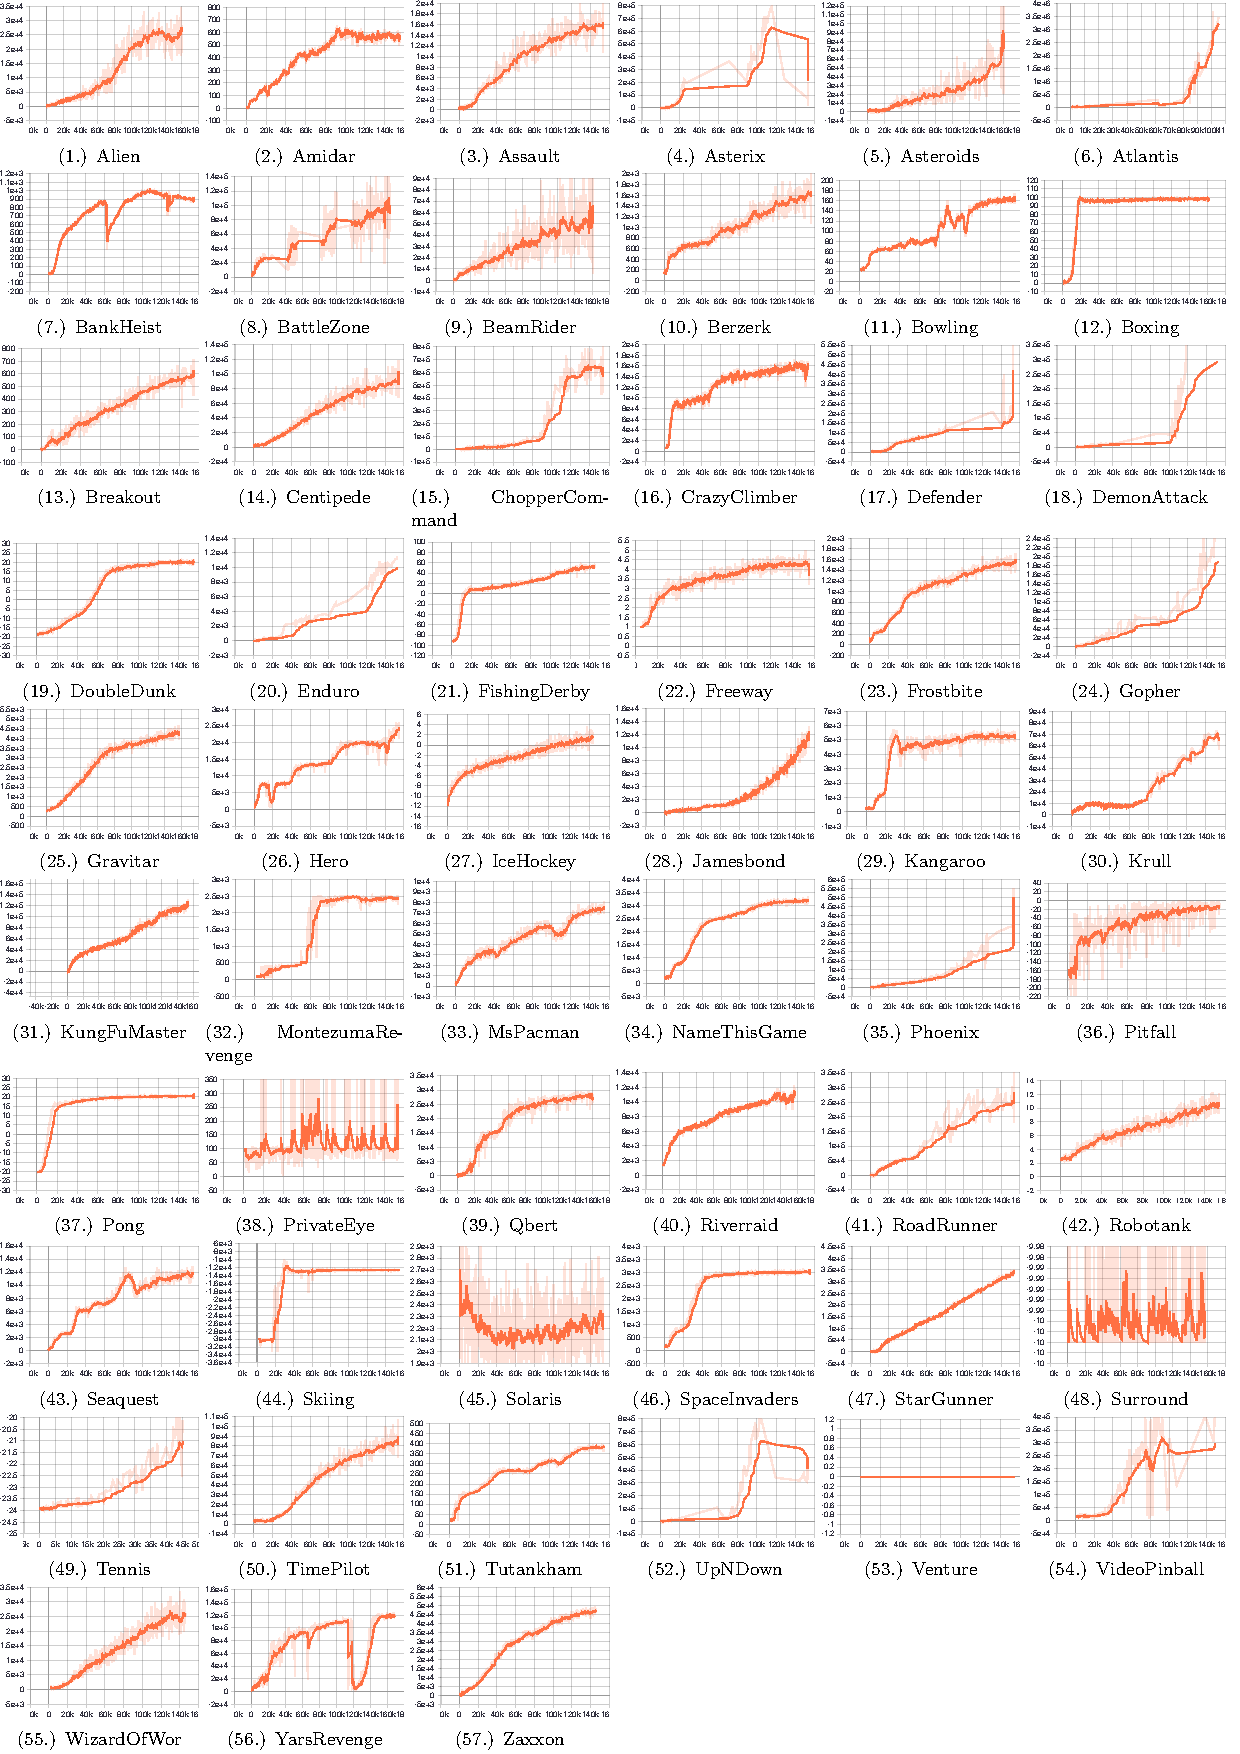
\includegraphics[width=1.0\linewidth]{body/all_fig3.pdf}
\end{figure*}

\clearpage



\end{document}
